\documentclass[14pt]{article}
\usepackage{geometry}                % See geometry.pdf to learn the layout options. There are lots.
\geometry{a4paper}                   % ... or a4paper or a5paper or ... 
\usepackage[english,russian]{babel}
\usepackage{graphicx}
\usepackage{amssymb}
\usepackage{amsmath}
\usepackage{epstopdf}
\usepackage{float}

\graphicspath{{./Fig/}}

\title{Библиотеки алгоритмов навигации и определения препятствий} 
\author{СК Роботикс }

\begin{document}
\maketitle

\section{Библиотека алгоритмов навигации - теория}

В состав библиотеки алгоритмов навигации входят следующие алгоритмы ориентации и навигации:

\begin{itemize}
    \item Алгоритм гирокомпассирования (Степан);
    \item Алгоритм курсовертикали, оценивающий ориентацию робота (углы курса, крена и тангажа) относительно навигационной системы координат (СК). В основе алгоритма лежит комплексирование информации от векторных датчика угловой скорости, магнитометра и акселерометра с использованием расширенного фильтра Калмана;
    \item Алгоритм навигации, вырабатывающий оценки координат, скоростей и азимутального угла ориентации робота относительно навигационной системы координат. Представлены две разновидности алгоритма, отличающиеся источником внешней информации, применяемой для корректирования оценок: с использованием измерений дальностей до локально установленных базовых станций радионавигационной системы UWB (Ultra-wide band, сверхширокополосная система малой мощности); с использованием измерений координат и скоростей, доставляемых глобальной спутниковой навигационной системой. Комплексирование в этих двух разновидностях комплексной системы навигации осуществляется с помощью расширенного фильтра Калмана;
     \item Алгоритм навигационной системы, комплексирующей измерения от локальной радионавигационной системы UWB с управляющими воздействиями, поступающими от системы траекторного управления колесного робота. Алгоритм обеспечивает оценку координат робота и его азимутального угла разворота относительно навигационной системы координат. Комплексирование  осуществляется с использованием нелинейного Байесовкого фильтра - фильтра частиц PF (particle filter).
\end{itemize} 

\subsection{Алгоритм гирокомпассирования}
Степан

\subsection{Алгоритм курсовертикали}
Задачей алгоритма курсовертикали  является определение углов ориентации колесного робота, в частности - азумутального угла разворота робота относительно навигационной СК.
Курсовертикаль включает три микромеханических датчика угловой скорости и три микромеханических акселерометра со взаимно ортогональными осями чувствительности.
Алгоритмически курсовертикаль построена на принципе коррекции ориентации, получаемой путем интегрирования  показаний датчиков угловой скорости.
Эта коррекция осуществляется по информации от векторных акселерометра и  магнитометра.

Комплексная обработка информации, используемая в алгоритме, основана на применении расширенного фильтра Калмана, оценивающего соответствующий вектор ошибок $\delta \boldsymbol x_M$. 
Определим состав  этого вектора. 
Уравнение ошибок $\delta\dot{\boldsymbol\Psi}^n$ ориентации, используемое в алгоритме курсовертикали:
\begin{equation}
 \delta\dot{\boldsymbol\Psi}^n = -C_b^n\delta\boldsymbol\omega^b.
\end{equation}

Уравнение измерений и модель ошибок измерений сформируем на примере определения вектора ускорения силы тяжести $\boldsymbol g^n$.
В случае равномерно и прямолинейно движущегося, либо неподвижного робота вектор $\boldsymbol g^n$ может быть записан так:
\begin{equation}\label{equ:acceleration_to_gravity}
\boldsymbol g^n = C_b^n \boldsymbol f^b,
\end{equation}
где $\boldsymbol f^b$ - вектор кажущегося ускорения, измеренный векторным акселерометром.
Для получения модели ошибок определения вектора ускорения силы тяжести проварьируем \eqref{equ:acceleration_to_gravity}:
Возмущенное значение $\tilde{\boldsymbol g}^n$ таково:
\begin{equation}
\boldsymbol{\tilde g}^n = \tilde{C}_b^n \tilde{\boldsymbol f}^b;
\end{equation}
\begin{equation}
\boldsymbol g^n + \delta \boldsymbol g^n = \left(I-E^n\right)C_b^n\left(\boldsymbol f^b+\delta\boldsymbol f^b\right);
\end{equation}
\begin{equation}\label{equ:acceleration_to_gravity_errors_raw}
\boldsymbol g^n + \delta \boldsymbol g^n = C_b^n \boldsymbol f^b + C_b^n \delta\boldsymbol f^b -  E^n C_b^n \boldsymbol f^b -E^nC_b^n  \delta\boldsymbol f^b.
\end{equation}

Удерживая в \eqref{equ:acceleration_to_gravity_errors_raw} только члены первого порядка малости, представим модель ошибок определения  вектора ускорения силы тяжести  так: 
\begin{equation}\label{equ:acceleration_to_gravity_errors_final}
\delta \boldsymbol g^n = C_b^n \delta\boldsymbol f^b + \left(\left[C_b^n \boldsymbol f^b\right]\times\right)  \delta\dot{\boldsymbol\Psi}^n.
\end{equation}

Вектор измерения $\boldsymbol z_{f}$ в канале коррекции курсовертикали с использованием акселерометра сформируем как разность оценки вектора ускорения силы тяжести $\hat{\boldsymbol g}^n$ (полученного с использованием соотношения типа \eqref{equ:acceleration_to_gravity}) и его эталонного значения ${\boldsymbol g}^n$:
\begin{equation}\label{equ:ahrs_measurements_start}
\boldsymbol z_f = \hat{\boldsymbol g}^n - {\boldsymbol g}^n = \delta \boldsymbol g^n. 
\end{equation}

С другой стороны, имеет место соотношение:
\begin{equation}
\boldsymbol z_f = H_f \delta \boldsymbol x_{M} + \boldsymbol\nu_f,
\end{equation}
где $H_f$ - матрица измерений в канале коррекции курсовертикали с использованием акселерометров; $\boldsymbol\nu_f$ - вектор шумов измерений.
Вектор ошибок курсовертикали $\delta \boldsymbol x_M$ определим следующим образом:
\begin{equation}\label{equ:ahrs_state}
\delta \boldsymbol x_M = \begin{bmatrix}\delta{\boldsymbol\Psi}^n & \delta\boldsymbol\omega^b  & \delta\boldsymbol f^b\end{bmatrix}^T.
\end{equation}

Из \eqref{equ:acceleration_to_gravity_errors_final}, \eqref{equ:ahrs_state} следует:
\begin{equation}
H_f = \begin{bmatrix}\left[C_b^n \boldsymbol f^b\right]\times & \boldsymbol 0 & C_b^n\end{bmatrix}.
\end{equation}
 
Отметим, что в общем случае для обеспечения  коррекции вычисленной курсовертикалью ориентации платформы недостаточно выполнить измерение направления одного вектора, в частности вектора ускорения силы тяжести $\boldsymbol g^n$, так как ориентация робота в плоскости, перпендикулярной этому вектору не определена, а ошибки ориентации по этой угловой координате - ненаблюдаемы.  
В качестве дополнительного вектора используем вектор магнитного поля Земли $\boldsymbol m^b$, измеряемый векторным магнитометром в связанной с роботом СК. 
Для этого вектора, по аналогии с вектором ускорения силы тяжести, соотношения для  модели измерения таковы:
\begin{equation}
\boldsymbol z_m = \hat{\boldsymbol m}^n - {\boldsymbol m}^n;
\end{equation}
\begin{equation}
\hat{\boldsymbol m}^n = \hat{C}_b^n \hat{\boldsymbol m}^b;
\end{equation}
\begin{equation}
\boldsymbol z_m = H_m \delta \boldsymbol x_{M} + \boldsymbol\nu_m;
\end{equation}
\begin{equation}\label{equ:ahrs_measurements_stop}
H_m = \begin{bmatrix}\left[C_b^n \boldsymbol m^b\right]\times & \boldsymbol 0 & \boldsymbol 0\end{bmatrix},
\end{equation}
где $\boldsymbol z_m$, $H_m$, $\boldsymbol\nu_m$ - соответственно вектор измерений, матрица измерений и вектор шумов измерений в канале коррекции курсовертикали с использованием магнитометра.
Полагая, что  динамика ошибок измерений $\delta \boldsymbol f^b$ и $\delta\boldsymbol\omega^b$ определяется соотношениями $\delta \dot{\boldsymbol f}^b = \boldsymbol n_f$  и $\delta \dot{\boldsymbol \omega}^b = \boldsymbol n_\omega$,  запишем уравнения ошибок курсовертикали в матричной форме  так:
\begin{equation}\label{equ:ahrs_errors_matrix}
\begin{bmatrix}
\delta\dot{\boldsymbol\Psi^n} \\ \delta \dot {\boldsymbol\omega}^b \\ \delta  \dot {\boldsymbol f}^b
\end{bmatrix}
 = 
\begin{bmatrix}
 \boldsymbol 0 & -C_b^n & \boldsymbol 0  \\
 \boldsymbol 0 & \boldsymbol 0 &\boldsymbol  0  \\
 \boldsymbol  0 & \boldsymbol 0 & \boldsymbol 0  
\end{bmatrix}
\begin{bmatrix}
\delta \boldsymbol\Psi^n \\ \delta \boldsymbol{\omega}^b \\ \delta  \boldsymbol{ f}^b
\end{bmatrix}
\begin{bmatrix}
\boldsymbol 0 & \boldsymbol 0 \\
I & \boldsymbol 0 \\
\boldsymbol 0 & I
\end{bmatrix}
\begin{bmatrix}
\boldsymbol n_{\omega} \\
\boldsymbol n_{f}
\end{bmatrix}
\end{equation}
где  $\boldsymbol n_\omega$  и $\boldsymbol n_f$ - белые шумы  гироскопов и акселерометров соответственно ($M\left[ \boldsymbol n_\omega \boldsymbol n_\omega^T\right] = Q_\omega\left(t\right)\delta\left(t-\tau\right)$, $M\left[ \boldsymbol n_f \boldsymbol n_f^T\right] = Q_f\left(t\right)\delta\left(t-\tau\right)$), $Q_\omega$ и $Q_f$ - матрицы интенсивностей белых шумов, $\delta\left(.\right)$ - дельта-функция).

Соотношения, приведенные выше, достаточны для формирования дискретного расширенного фильтра Калмана.
Результатом работы алгоритма курсовертикали являются оценки ориентации робота, сдвигов нулей датчиков угловой скорости и векторного акселерометра. 

\subsubsection{Моделирование работы алгоритма курсовертикали}
Для оценки точности работы алгоритма курсовертикали проведено моделирование в рамках которого задается опорное движение твердого тела с курсовертикалью с помощью алгоритма SPIN-CONE, синтезирующего кинематические параметры тела, вращающегося с постоянной угловой скоростью вокруг некоторой оси вращения, которая в свою очередь описывает конус вокруг оси прецесии с постоянной угловой скоростью прецесии. 
На Рис. \ref{fig:ahrs_angle} - \ref{fig:ahrs_bias} приведены результаты моделирования работы алгоритма курсовертикали демонстрирующие сходящийся процесс оценивания ошибок углов ориентации и состоятельные оценки сдвигов нулей гироскопов. 

\begin{figure}
\noindent\centering{
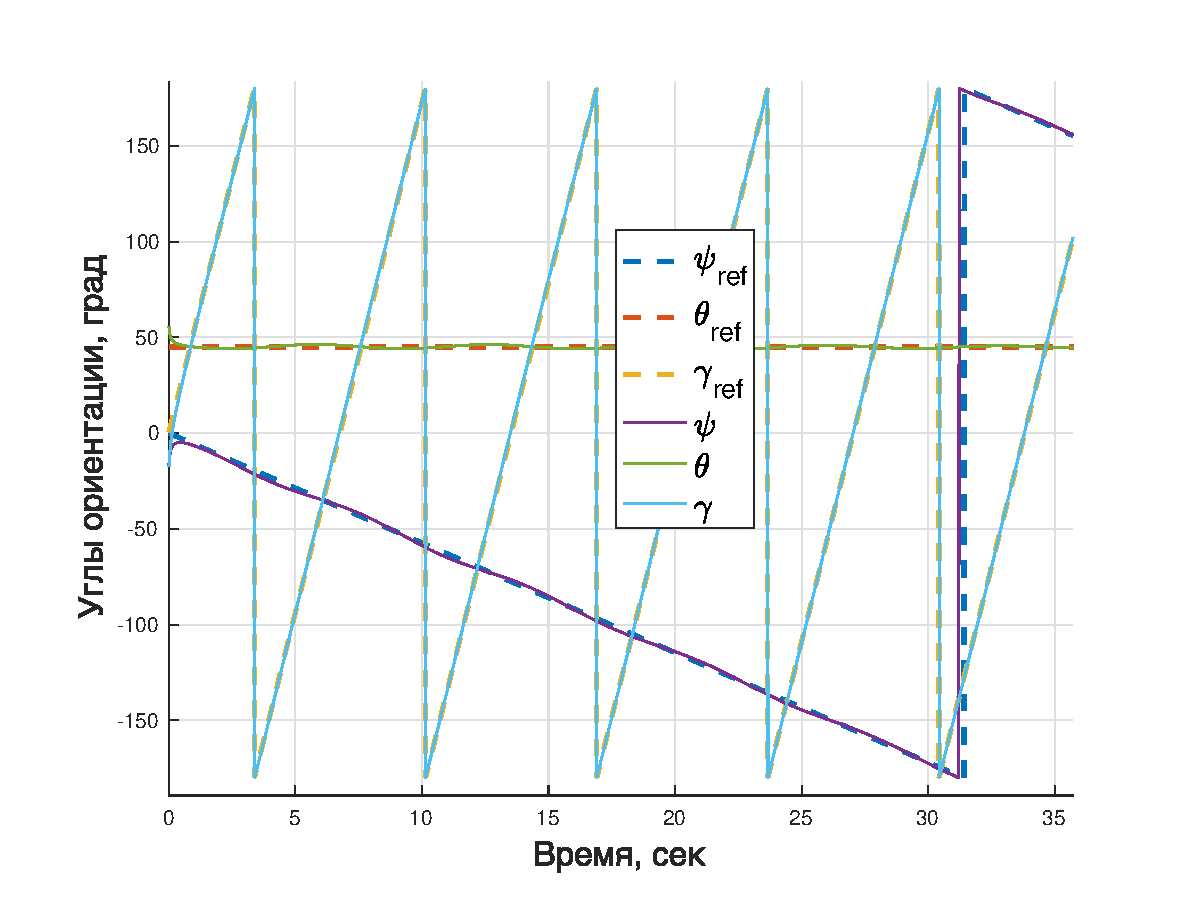
\includegraphics[width=120mm]{ahrs_angle.eps}
}
\caption{Опорные углы ориентации и их оценки алгоритмом курсовертикали}
\label{fig:ahrs_angle}
\end{figure}

\begin{figure}
\noindent\centering{
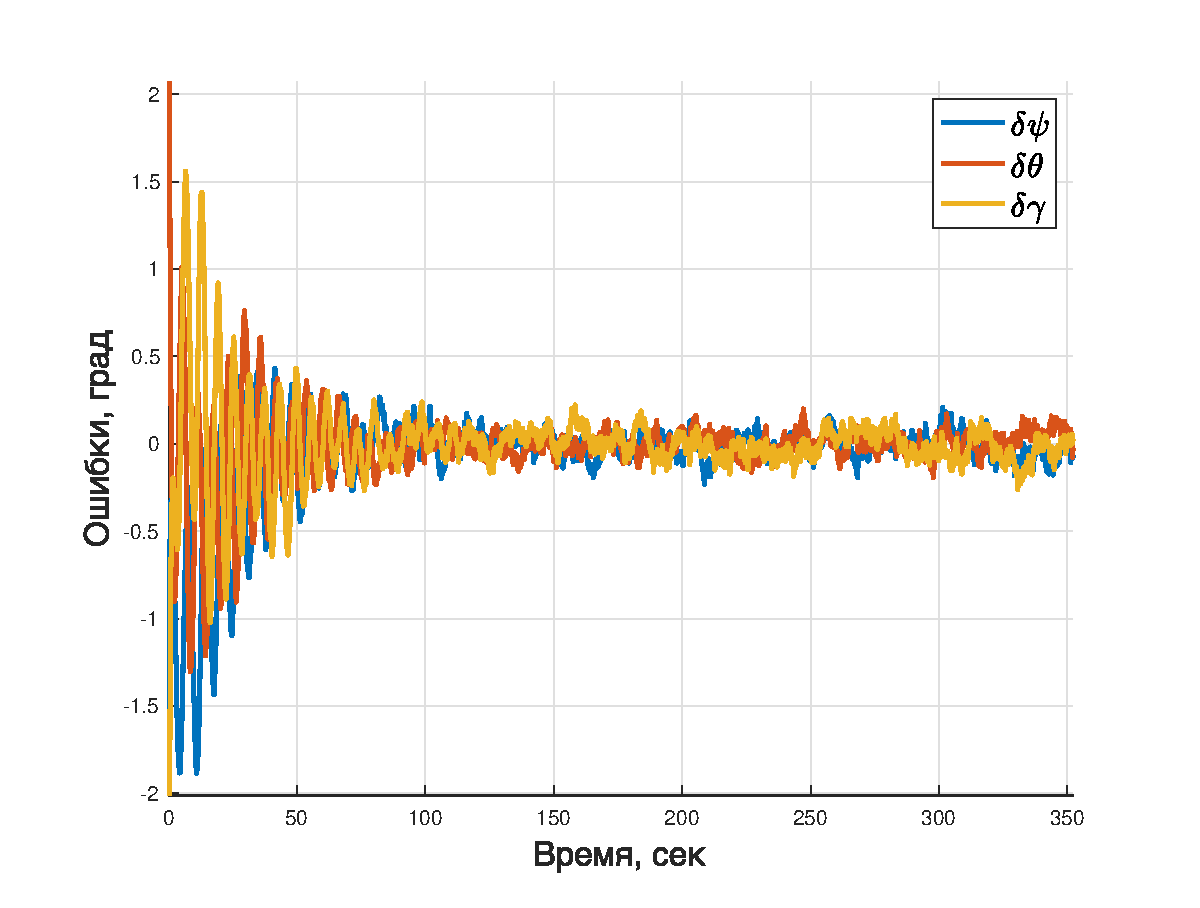
\includegraphics[width=120mm]{ahrs_angle_errors.eps}
}
\caption{Ошибки оценок углов ориентации алгоритмом курсовертикали}
\label{fig:ahrs_angle_errors}
\end{figure}

\begin{figure}
\noindent\centering{
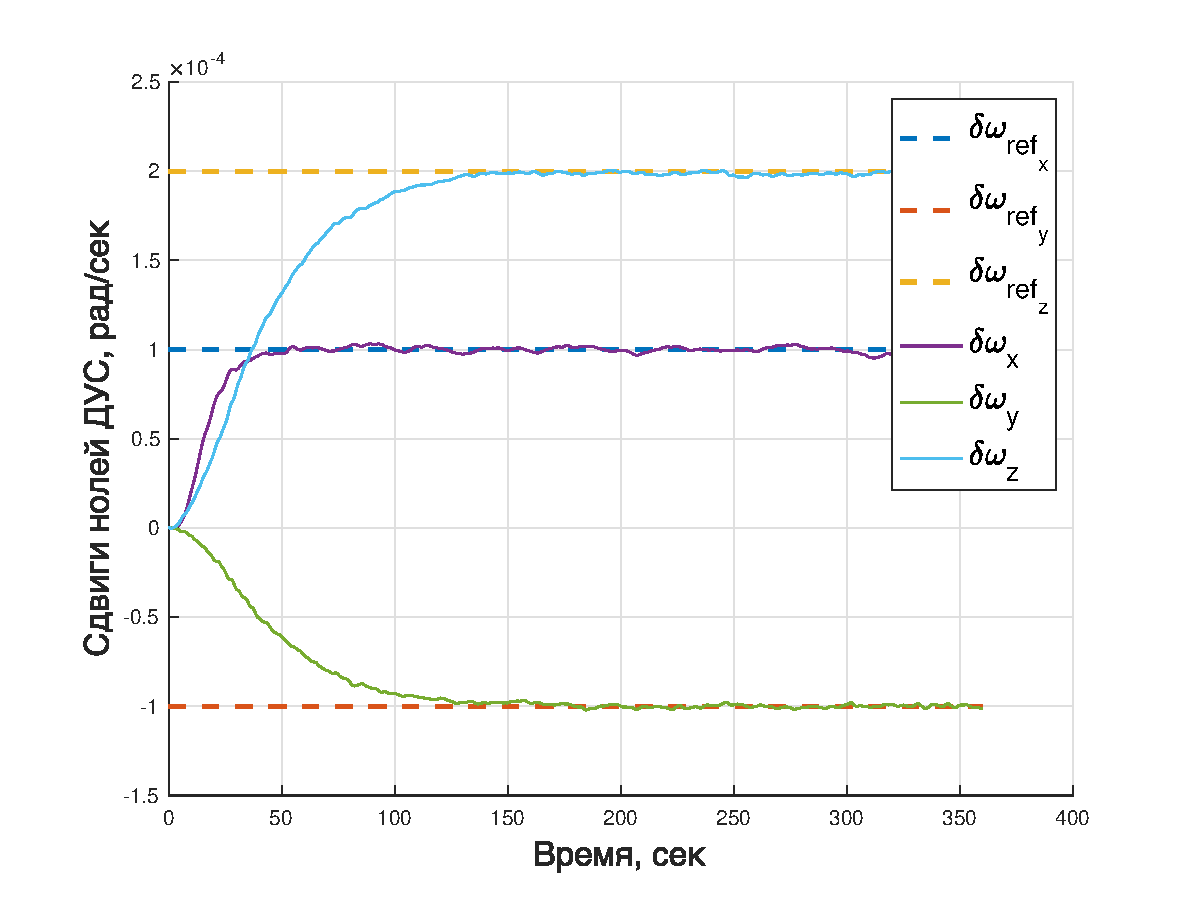
\includegraphics[width=120mm]{ahrs_bias.eps}
}
\caption{Оценки сдвигов нолей ДУС алгоритмом курсовертикали}
\label{fig:ahrs_bias}
\end{figure}

\clearpage

\subsection{Алгоритм комплексной системы навигации с использованием расширенного фильтра Калмана}

\subsubsection{Алгоритм навигации с коррекцией от UWB}

Комплексная система навигации трехколесного робота с двумя ведущими колесами и третьим пассивным поддерживающим колесом включает датчики скоростей вращения ведущих правого и левого колес, датчик угловой скорости вращения робота вокруг его вертикальной оси. Использование этих источников информации позволяет оценивать координаты, скорости и угол курса робота в навигационной системе координат. Однако, непрерывное интегрирование  сигналов датчиков приводит к неконтролируемому нарастанию во времени ошибок определенеия навигационных параметров робота.

Для компенсации этих ошибок и получения стабильного навигационного решения традиционно используется приемник глобальной навигационной спутниковой системы (ГНСС), информация от которого о координатах и скоростях носителя комплексируются с информацией от одометра и курсового гироскопа. При этом среда, в которой функционирует мобильный робот, зачастую включает помещения, например, ангары, внутри которых получение стабильного навигационного решения приемником ГНСС затруднено.

Для организации непрерывного, корректирующего локального навигационного поля в работе предложено использовать измерения от локальной радионавигационной системы на базе ультраширокополосной технологии ultra-wide band (UWB). Эта радиочастотная технология использует короткие импульсы с максимально возможной полосой пропускания при минимально возможной центральной частоте. Технология используется в устройствах связи, радиолокации, при определении расстояний и позиционировании.

В состав локальной радионавигационной системы входит мобильный приемо-передатчик сигналов, устанавливаемый на трехколесном поботе и несколько стационарных базовых станций, устанавливаемых на обьекте, в рамках которого необходимо осуществлять навигацию робота. В результате двустороннего обмена короткими широковещательными радиопакетами между приемо-передатчиком и базовой станцией происходит синхронизация времени на субнаносекундном уровне, что позволяет определеть время распостранения радоисигнала и, как следствие, вычислить расстояние между этими двумя устройствами с сантиметровой точностью. 

Таким образом, в предлагаемой комплексной системе навигации предлагается выполнить сильно связанное комплексирование информации от нескольких разнородных источников - одометра, датчика угловой скорости, локальной системы UWB с целью получения точного и робастного навигационного решения.

На Рис. \ref{fig:uwb_intergated_axes} показаны связанная и навигационная системы координат, схематично приведены расположение элементов системы UWB на роботе и на обьекте, в рамках которого предполагается осуществлять навигацию. Координаты базовых станций UWB в навигационной системе координат считаются фиксированными и известными. 

\begin{figure}
\noindent\centering{
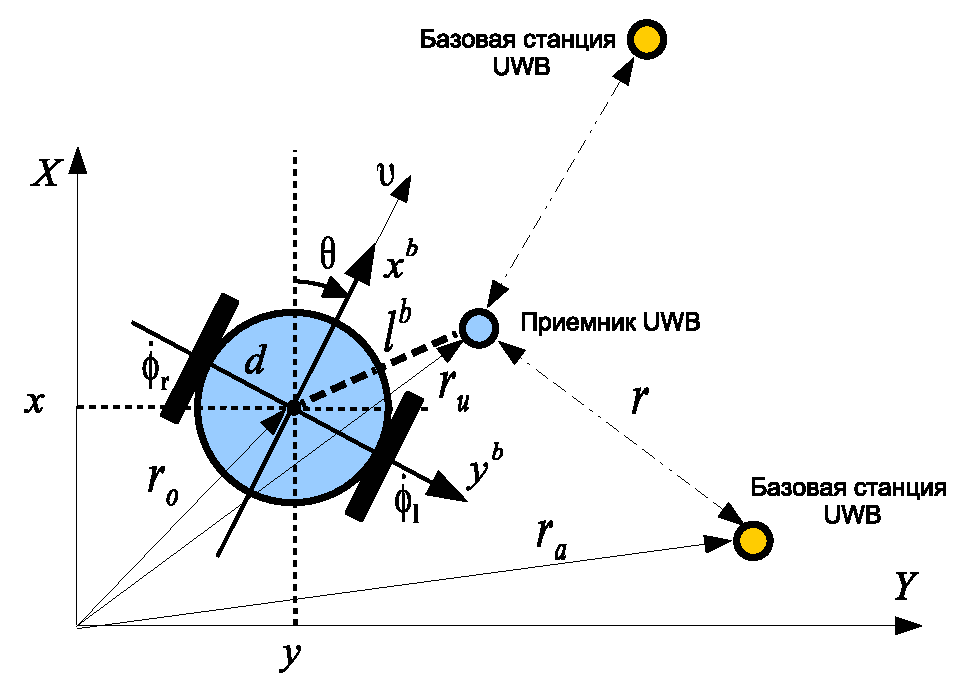
\includegraphics[width=120mm]{axes_uwb.eps}
}
\caption{Система координат}
\label{fig:uwb_intergated_axes}
\end{figure}

Уравнения одометра:
\begin{equation}
\upsilon_x^b = \frac{1}{2}(\dot{\phi}_r l_r+\dot{\phi}_l l_l);
\end{equation}
\begin{equation}
\dot\theta = \frac{1}{d}(\dot{\phi}_r l_r-\dot{\phi}_l l_l),
\end{equation}
где: $\upsilon_x^b$ - продольная скорость перемещения робота;  $\dot\theta$ - угловая скорость разворота робота вокруг вертикальной оси;  $\dot{\phi}_r,\dot{\phi}_l$ - угловые скорости вращения правого и левого колес; $l_r, l_l$ - длины окружностей колес; $d$- длина оси колесной пары.

Угловые скорости вращения колес могут в свою очередь быть получены на основе скорости продольного перемешения и скорости разворота вокруг вертикальной оси следующим образом:
\begin{equation}
\dot{\phi}_r = \frac{\upsilon_x^b}{l_r}+\frac{\dot\theta d}{2 l_r};
\end{equation}
\begin{equation}
\dot{\phi}_l = \frac{\upsilon_x^b}{l_r}-\frac{\dot\theta d}{2 l_r}.
\end{equation}

Уравнения навигации:
\begin{equation}
\dot{r}^n=C_b^n\upsilon^b=C_b^n \begin{bmatrix}\upsilon_x^b & 0 & 0 \end{bmatrix}^T;
\end{equation}
 
\begin{equation}
\dot{C}_b^n = C_b^n\Omega^b;
\end{equation}

\begin{equation}
C_b^n = \begin{bmatrix}\cos\theta & -\sin\theta\ & 0 \\ \sin\theta & \cos\theta & 0 \\ 0 & 0 &1 \end{bmatrix},
\end{equation}

где: $\Omega^b$ - кососимметричная матрица вектора $\omega^b=\begin{bmatrix}0 & 0 & \omega_z\end{bmatrix}^T$, $\omega_z$ - измерение датчика угловой скорости;  $r^n = r_o= \begin{bmatrix}x&y&0\end{bmatrix}^T$ - координаты центра оси колес в навигационной системе координат.

Уравнения ошибок одометра (ошибок определения скорости продольного перемещения $\delta\upsilon_x^b$ и скорости разворота по углу курса $\delta\dot\theta$):
\begin{equation}
\delta\upsilon_x^b = \cfrac{1}{2}\left(\dot{\phi}_r \delta l_r+\dot{\phi}_l \delta l_l\right);
\end{equation}
\begin{equation}
\delta\dot\theta = \cfrac{1}{d}\dot{\phi}_r \delta l_r-\cfrac{1}{d}\dot{\phi}_l \delta l_l+\cfrac{1}{d^2}\left(\dot{\phi}_l  l_l-\dot{\phi}_r l_r\right)\delta d;
\end{equation}
где: $\delta l_l, \delta l_l$ - ошибки определения длины окружностей колес; $\delta d$-ошибка определения длины оси колесной пары.

Динамика ошибок координат, ориентации и слвига нуля датчика угловой скорости 
\begin{equation}
\delta\dot{r}^n=C_b^n\delta\upsilon^b+\left(\left[C_b^n\upsilon^b\right]\times\right)\delta\psi^n;
\end{equation}
\begin{equation}
\delta\dot{\psi}^n=-C_b^n\delta\omega^b;
\end{equation}
\begin{equation}
\delta\dot{\omega}^b=n_\omega;
\end{equation}
где: $\delta r^n=\begin{bmatrix}\delta x&\delta y&0\end{bmatrix}$ - вектор ошибок координат; $\delta\upsilon^b=\begin{bmatrix}\delta\upsilon_x^b&0&0\end{bmatrix}^T$-вектор ошибок скорости; $\delta\psi^n=\begin{bmatrix}0&0&\delta\psi^n_z\end{bmatrix}$  - вектор ошибок ориентации; $n_w$ - шум датчика угловой скорости.

Координаты $r_u$ приемника системы UWB, расположенного на роботе, могут быть записаны так:
\begin{equation}
r_u = r_o+C_b^nl^b
\end{equation}
где: $r_o=r^n$ -  координаты центра оси колесной пары; $l^b = \begin{bmatrix}l^b_x&l^b_y&0\end{bmatrix}^T$ - вектор смещения точки закрепления приемника UWB относительно центра оси колесной пары.

Измерение расстояния $||r||_2$ между стационарной базовой станцией и мобильным приемником, закрепленным на роботе может быть записано так:
\begin{equation}
   ||r||_2 = ||r_a-r_u||_2=||r_a-r_o-C_b^n l^b||_2
\end{equation}
 \begin{equation}
   ||r||_2^2 = \left[r_a-r_o-C_b^n l^b\right]^T\left[r_a-r_o-C_b^n l^b\right]
\end{equation}

Проварьируем уравнение измерений (15):
\begin{align}
   2r\delta r=&\left[r_a -r_o-\delta r_o-\left(I-E^n\right)C_b^n\left(l^b+\delta l^b\right)\right]^T \\ &\left[r_a - r_o-\delta r_o-\left(I-E^n\right)C_b^n\left(l^b+\delta l^b\right)\right]
\end{align}

Тогда ошибку измерения $ \delta r$ расстояния $r$ можно записать через ошибки определения координат, ориентации, размещения  приемника  UWB так:
 \begin{align}
   \delta r &= \left(r_o^T-r_a^T+\left(l^b\right)^TC_n^b\right)  \delta r_o+\\&+\left((l^b)^T+\left(r_o^T-r_a^T\right)C_b^n\right)\delta l^b+\\&+\left(r_o^T-r_a^T+  \left(l^b\right)^TC_n^b\right)\left(\left[C_b^nl^b\right]\times\right)\delta\psi^n
\end{align}

Комплексирование навигационной информации от всех источников осуществляется с использованием расширенного фильтра Калмана который оценивает компоненты следующего вектора ошибок навигационной системы трехколесного робота:
\begin{equation}
 \mathbf x = \begin{bmatrix}\delta x & \delta y & \delta\psi^n_x & \delta l_r & \delta l_l & \delta\omega_z & \delta d & \delta l^b_x & \delta l^b_y  \end{bmatrix}^T
 \end{equation}
   
Вектор и матрица измерений системы UWB:
\begin{equation}
 \mathbf z = \begin{bmatrix}\hat r-r\end{bmatrix}
 \end{equation}
   
\begin{equation}
\mathbf H = \begin{bmatrix} 
r_o^T-r_a^T+\left(l^b\right)^TC_n^b \\ \left(r_o^T-r_a^T+\left(l^b\right)^TC_n^b\right)\left(\left[C_b^nl^b\right]\times\right)  \\ 0_{4 \times 1} \\ \left(l^b\right)^T+\left(r_o^T-r_a^T\right)C_b^n 
\end{bmatrix}^T
\end{equation}

Вектор и матрица измерений одометра (датчики угловой скорости вращения ведущих колес и курсового гироскопа):
 \begin{equation}
   \mathbf z = \begin{bmatrix}\hat{\omega}_z-\dot\theta\end{bmatrix}
 \end{equation}
   
\begin{equation}
   \mathbf H = \begin{bmatrix} 0 & 0 & 0 & -\cfrac{\dot\phi_r}{d} & \cfrac{\dot\phi_l}{d} & 1 & \cfrac{1}{d^2}\left(\dot{\phi}_r  l_r-\dot{\phi}_l l_l\right) & 0 & 0 & 0 \end{bmatrix}
\end{equation}

\subsubsection{Моделирование работы алгоритма навигации с коррекцией от UWB}
С целью оценки точности и устойчивости работы комплексной системы навигации был проведен численный эксперимент в котором моделировалось перемещение робота с комплексной системой навигации по замкнутой траектории в рамках покрытия локальной радионавигационной системы UWB с четырьмя базовыми станциями, расположенными так, как показано на Рис. \ref{fig:uwb_intergated_trajectory}. 

\begin{figure}
\noindent\centering{
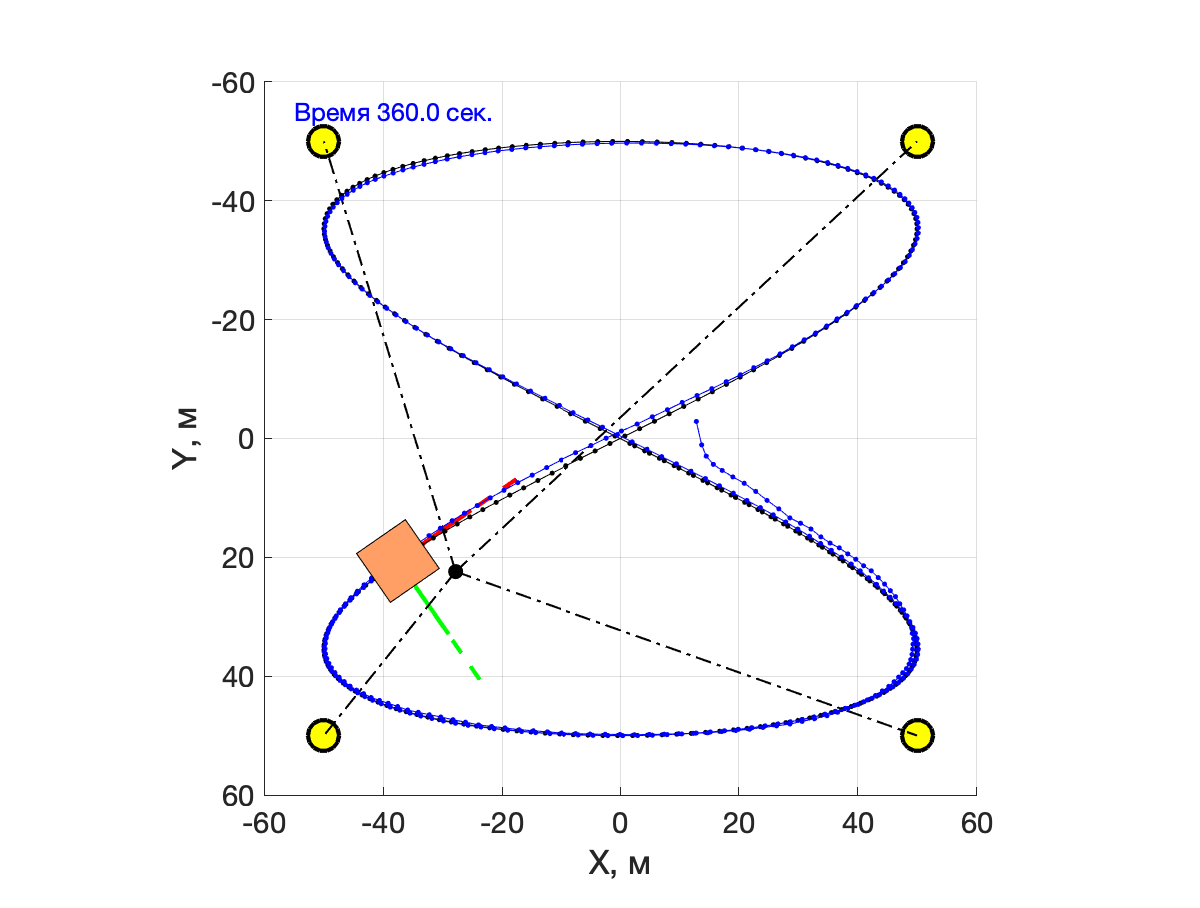
\includegraphics[width=120mm]{trajectory.eps}
}
\caption{Модельная траектория и расположение базовых станций UWB}
\label{fig:uwb_intergated_trajectory}
\end{figure}

 В результате моделирования продемонстрирована устойчивая работа навигационного комплекса трехколесного робота. На рисунках \ref{fig:uwb_coordinates} - \ref{fig:uwb_lever} приведены результаты моделирования. 
 
\begin{figure}
\noindent\centering{
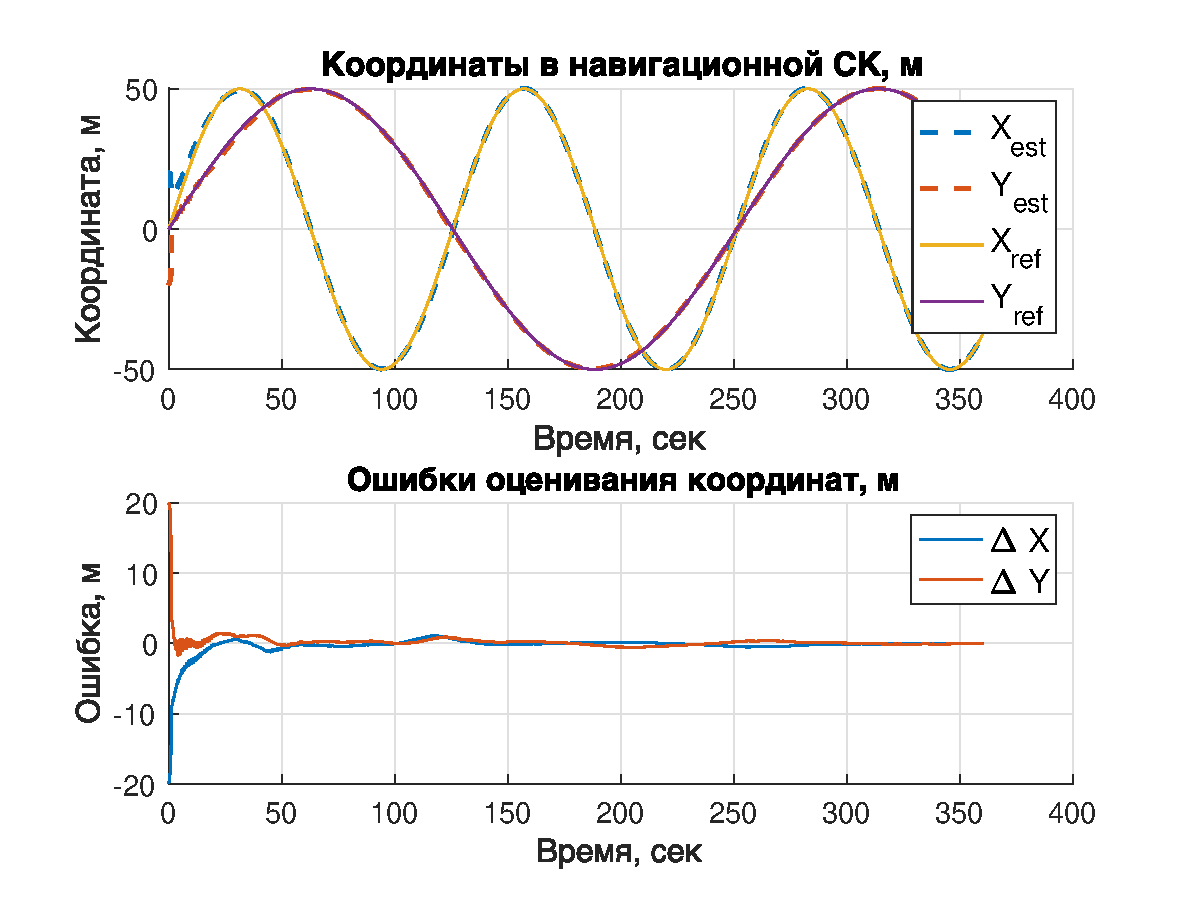
\includegraphics[width=120mm]{position.eps}
}
\caption{Координаты робота и оценки их ошибок - UWB коррекция}
\label{fig:uwb_coordinates}
\end{figure}

\begin{figure}
\noindent\centering{
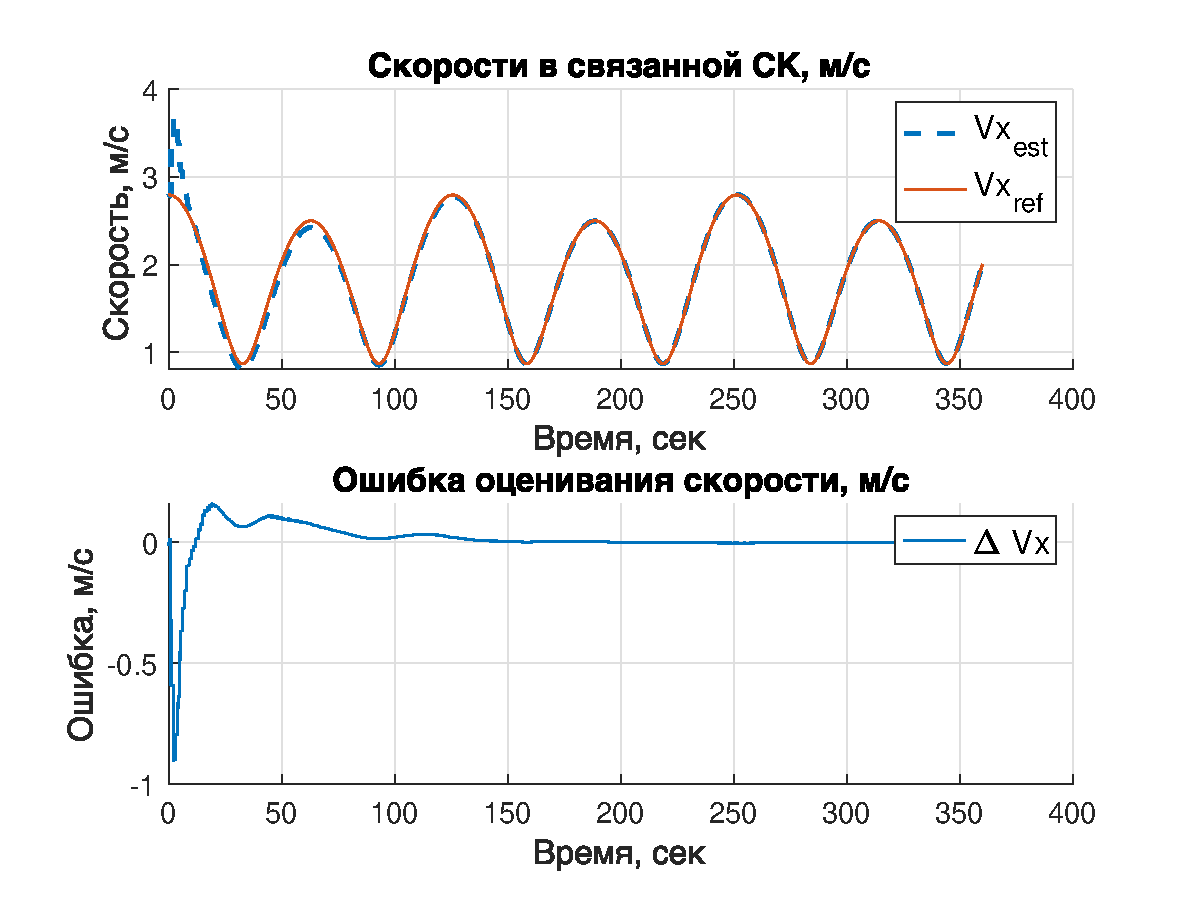
\includegraphics[width=120mm]{velocity.eps}
}
\caption{Скорость продольного перемещения робота и оценка ее ошибки - UWB коррекция}
\label{fig:uwb_velocities}
\end{figure}

\begin{figure}
\noindent\centering{
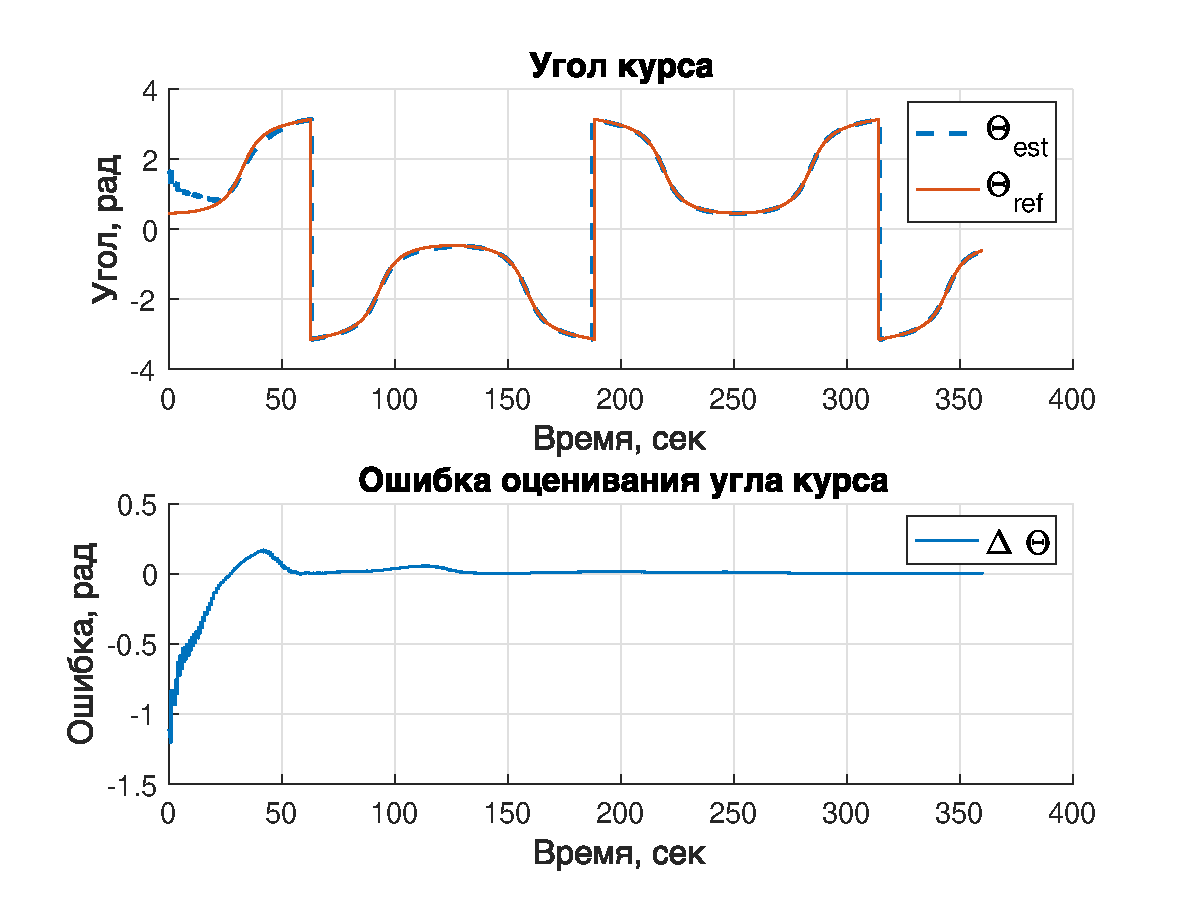
\includegraphics[width=120mm]{heading.eps}
}
\caption{Угол курса робота и  оценка его ошибки - UWB коррекция}
\label{fig:uwb_heading}
\end{figure}

\begin{figure}
\noindent\centering{
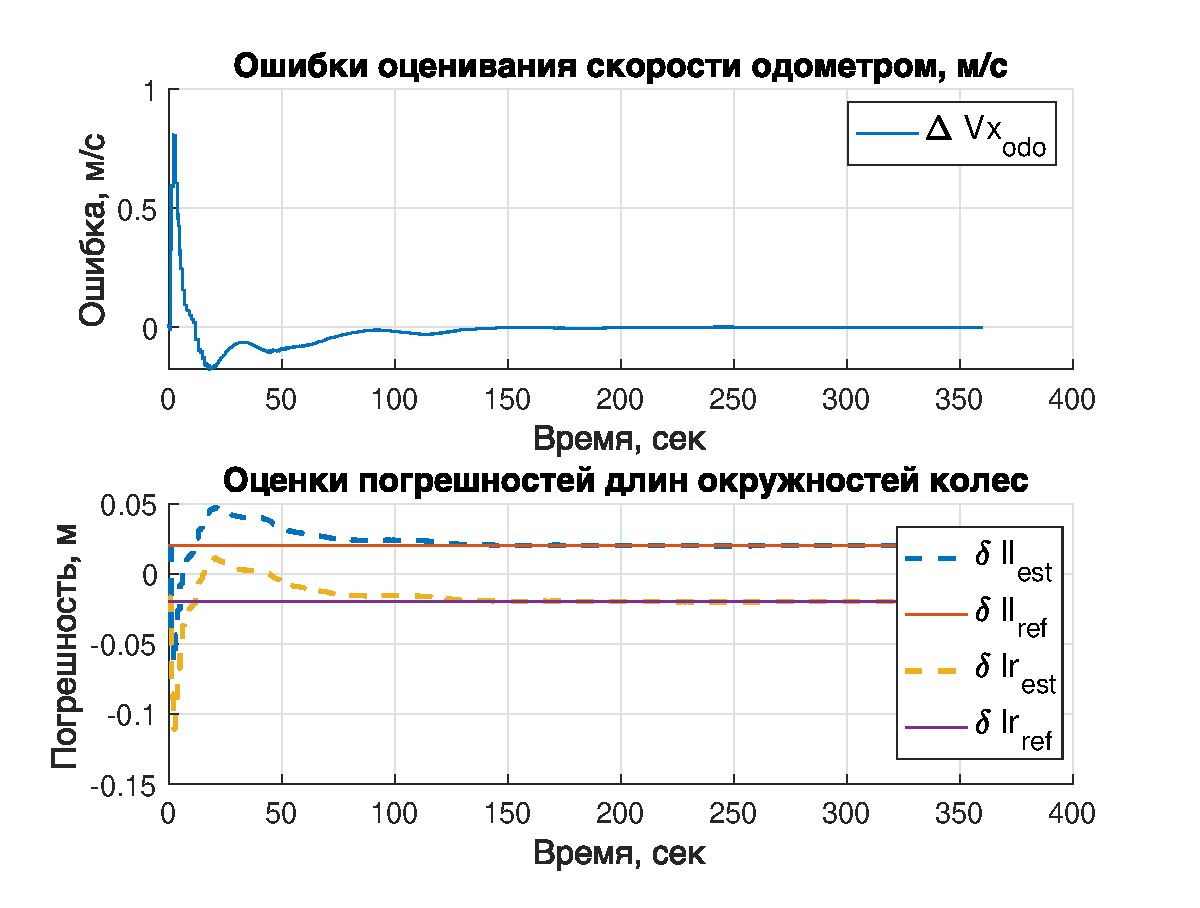
\includegraphics[width=120mm]{errors_odo.eps}
}
\caption{Оценка ошибок одометра - UWB коррекция}
\label{fig:uwb_odometer}
\end{figure}

\begin{figure}
\noindent\centering{
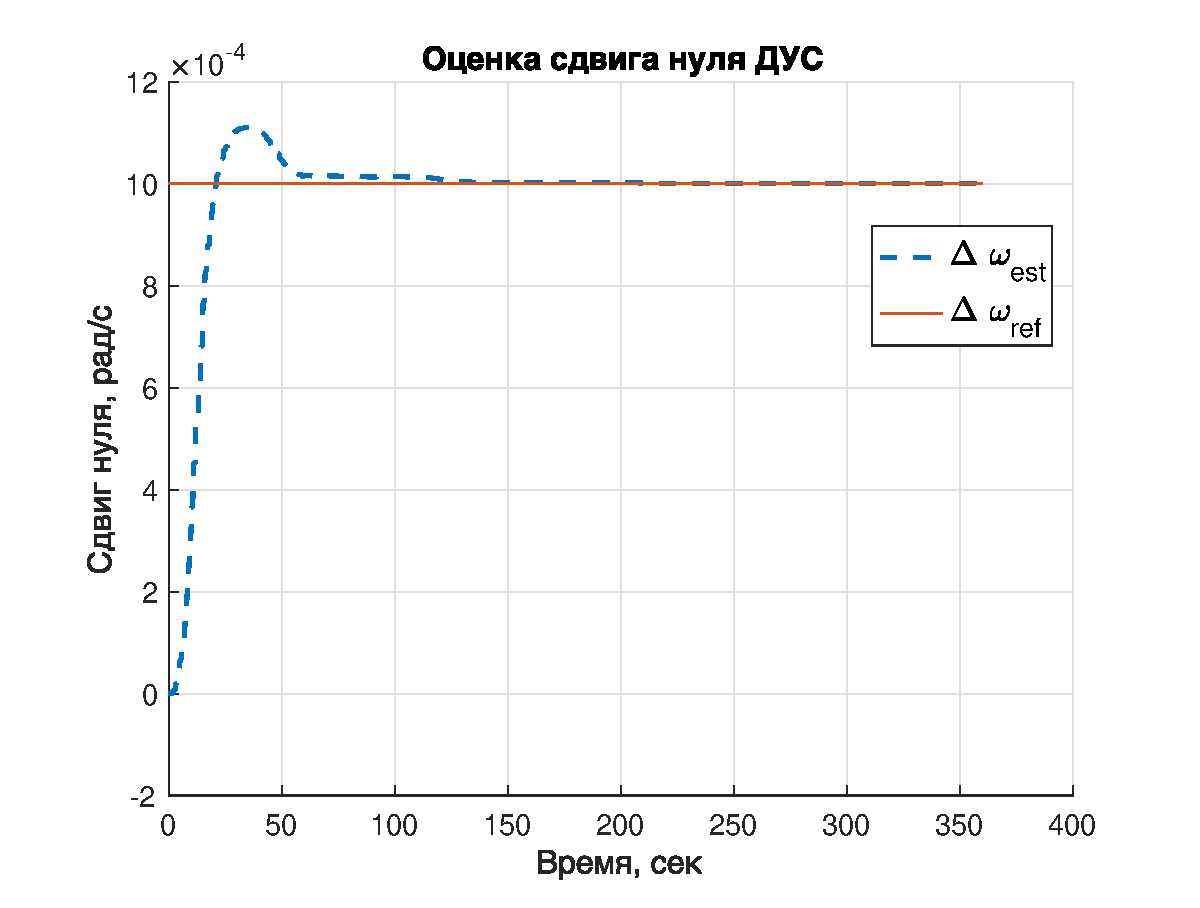
\includegraphics[width=120mm]{errors_gyro.eps}
}
\caption{Оценка ошибок датчика угловой скорости - UWB коррекция}
\label{fig:uwb_gyro_bias}
\end{figure}

\begin{figure}
\noindent\centering{
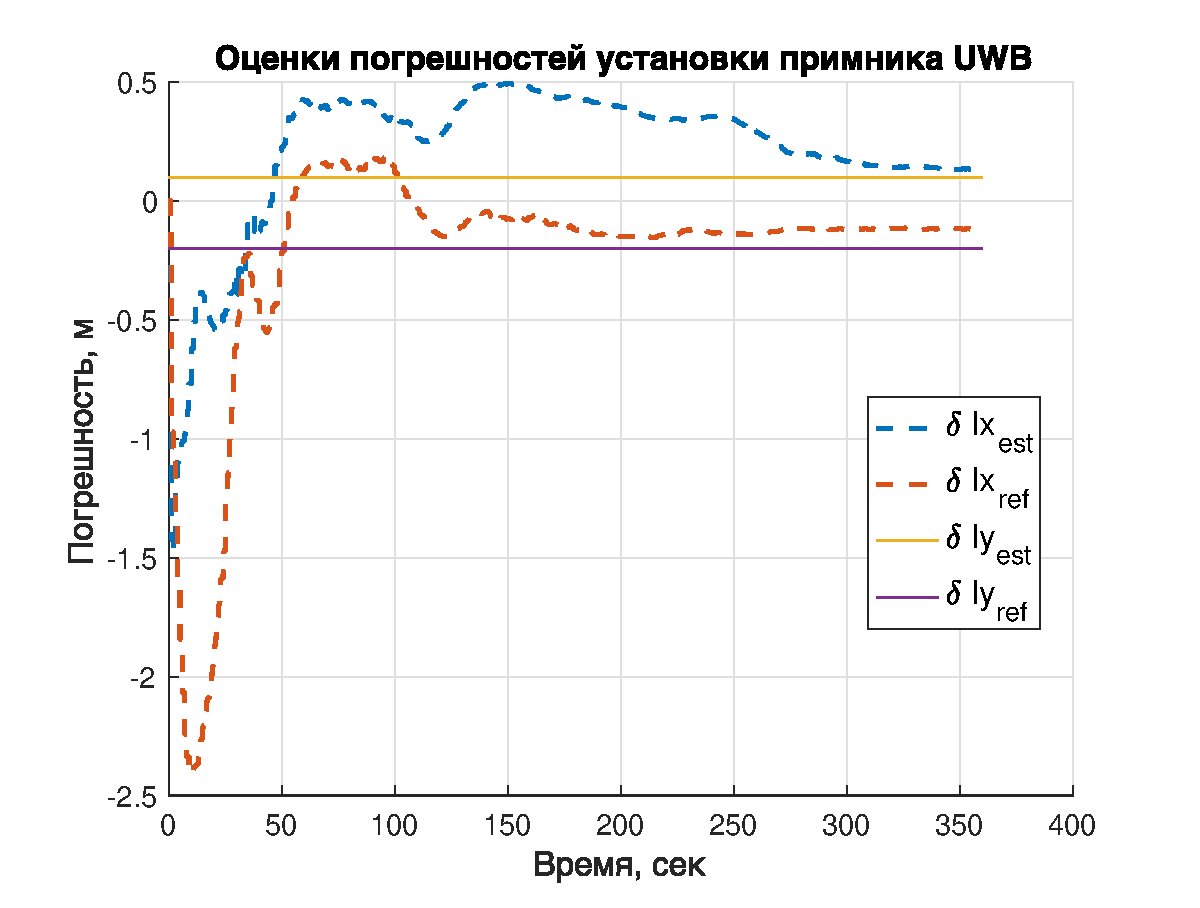
\includegraphics[width=120mm]{errors_lever.eps}
}
\caption{Оценка погрешностей установки приемника UWB}
\label{fig:uwb_lever}
\end{figure}

\clearpage

\subsubsection{Алгоритм навигации с коррекцией от спутниковой навигационной системы}
В этом варианте алгоритма система координат (Рис. \ref{fig:uwb_intergated_axes}) и структура системы остается прежней, с той только разницей, что приемник системы UWB заменяется на приемник  спутниковой навигационной системы.

Комплексирование навигационной информации в этом случае также осуществляется с использованием расширенного фильтра Калмана который оценивает компоненты следующего вектора ошибок навигационной системы трехколесного робота:
\begin{equation}
 \mathbf x = \begin{bmatrix}\delta x & \delta y & \delta\psi^n_x & \delta l_r & \delta l_l & \delta\omega^b_z  \end{bmatrix}^T
 \label{equ:state_gps}
 \end{equation}
   
Вектор и матрица измерений при использовании в качестве корректирующей спутниковой системы навигации (СНС):
\begin{equation}
 \mathbf z = \begin{bmatrix} {\hat r}^n_{снс} - r^n_{снс} \\ {\hat \upsilon}^n_{снс} - \upsilon^n_{снс} \end{bmatrix},
 \end{equation}
 
 где ${\hat r}^n_{снс}$, ${\hat \upsilon}^n_{снс}$ - оценки векторов координат и скоростей приемника СНС в навигационной СК, формируемые так:
 
 \begin{equation}
  {\hat r}^n_{снс} = r_o + C_b^n l^b
 \end{equation}
 
 \begin{equation}
  {\hat \upsilon}^n_{снс} =  C_b^n \left(\upsilon^b + \left[\omega^b\times\right] l^b\right)
 \end{equation}
 
 Ошибки оценок координат и скоростей премника СНС можно записать следующим образом:
 
 \begin{equation}
  \delta r^n = \delta r_o  +  \left[ C_b^n l^b \times \right]\delta\psi^n 
  \label{equ:error_pos_gps}
 \end{equation}
   
 \begin{equation}
  \delta\upsilon^n = - C_b^n \left[l^b\times\right]\delta\omega^b + \left[\left(C_b^n\upsilon^b+C_b^n\left[\omega^b\times\right] l^b\right)\times\right]\delta\psi^n 
  \label{equ:error_vel_gps}
 \end{equation}

Вид матрицы измерений $H$ расширенного фильтра Калмана однозначным образом следует из \eqref{equ:state_gps},  \eqref{equ:error_pos_gps}, \eqref{equ:error_vel_gps}.

\subsubsection{Моделирование работы алгоритма навигации с коррекцией от СНС}
С целью демонстрации работы работы алгоритма комплексной системы навигации с коррекцией от СНС было провелено его моделирование в рамках которого было задано перемещение модели робота по траектории, аналогичной приведенной на Рис. \ref{fig:uwb_intergated_trajectory}. На рисунках \ref{fig:gps_coordinates} - \ref{fig:gps_gyro_bias} приведены результаты моделирования, демонстрирующие устойчивость и точность работы алгоритма комплекной системы навигации.

\begin{figure}
\noindent\centering{
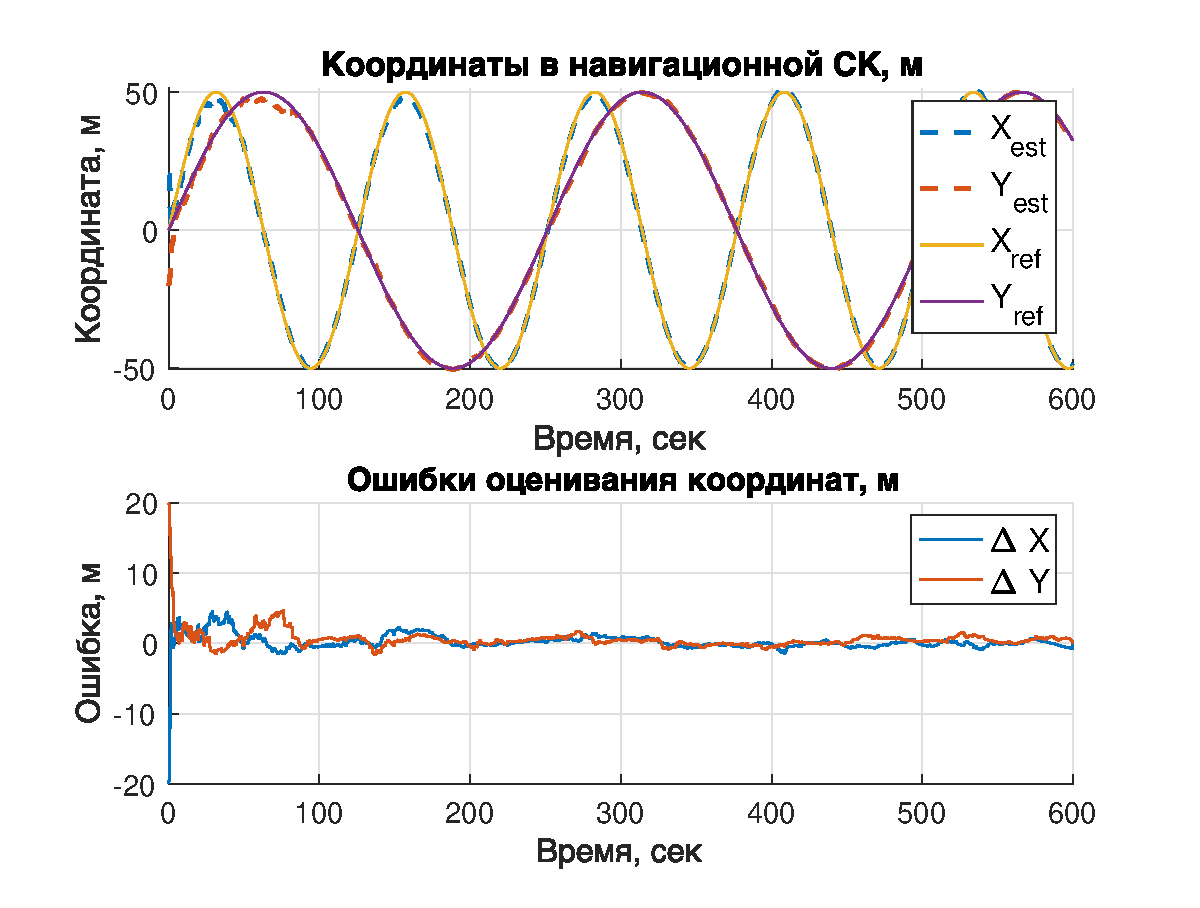
\includegraphics[width=120mm]{gps_position.eps}
}
\caption{Координаты робота и оценки их ошибок - СНС коррекция}
\label{fig:gps_coordinates}
\end{figure}

\begin{figure}
\noindent\centering{
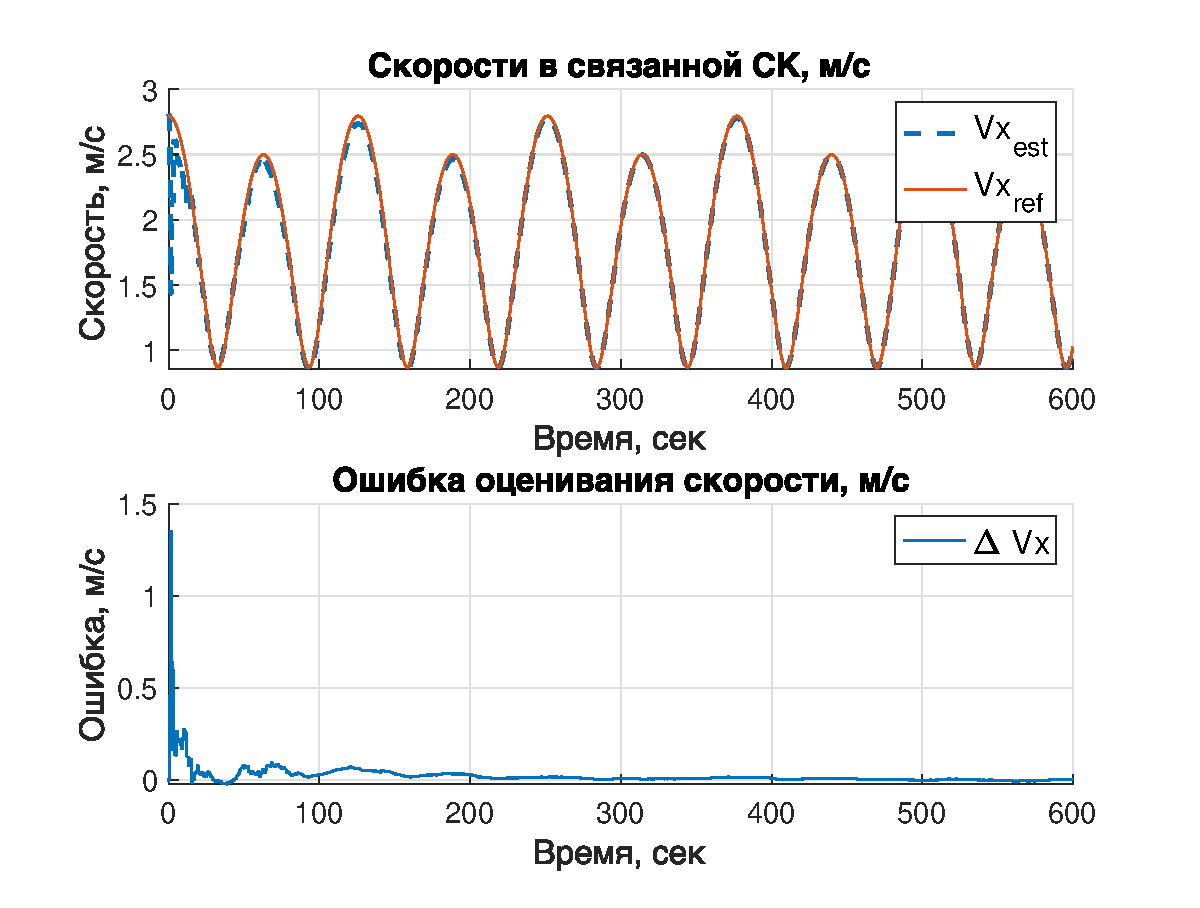
\includegraphics[width=120mm]{gps_velocity.eps}
}
\caption{Скорость продольного перемещения робота и оценка ее ошибки - СНС коррекция}
\label{fig:gps_velocities}
\end{figure}

\begin{figure}
\noindent\centering{
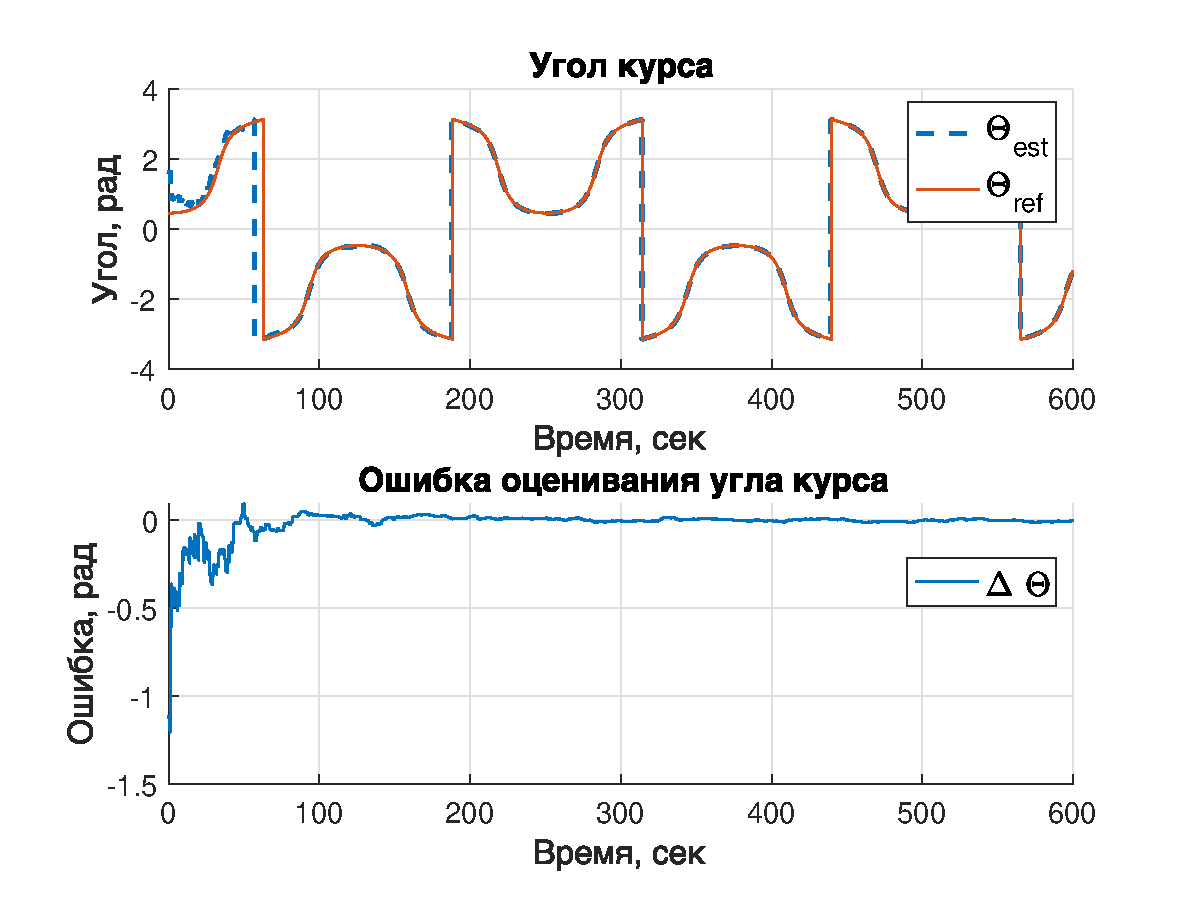
\includegraphics[width=120mm]{gps_heading.eps}
}
\caption{Угол курса робота и  оценка его ошибки - СНС коррекция}
\label{fig:gps_heading}
\end{figure}

\begin{figure}
\noindent\centering{
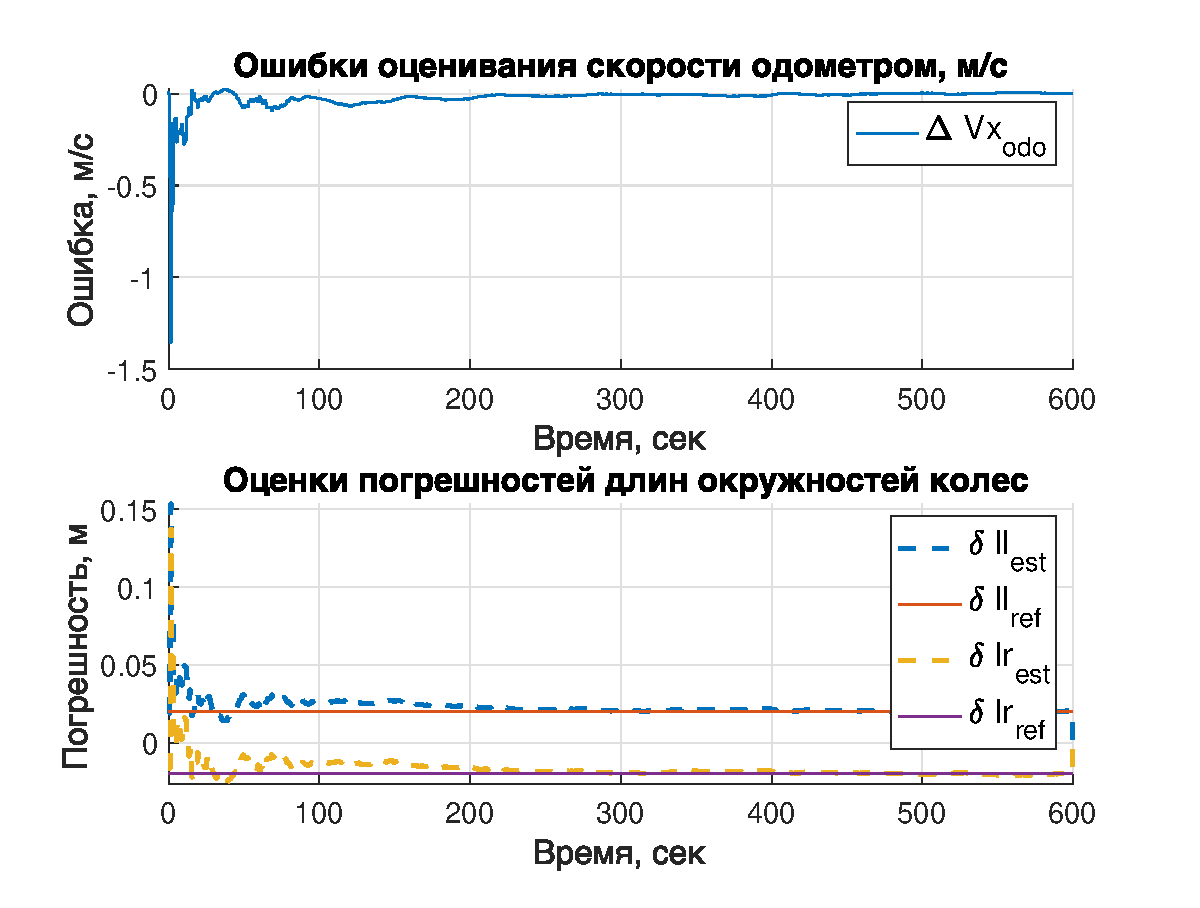
\includegraphics[width=120mm]{gps_odometer_bias.eps}
}
\caption{Оценка ошибок одометра - СНС коррекция}
\label{fig:gps_odometer}
\end{figure}

\begin{figure}
\noindent\centering{
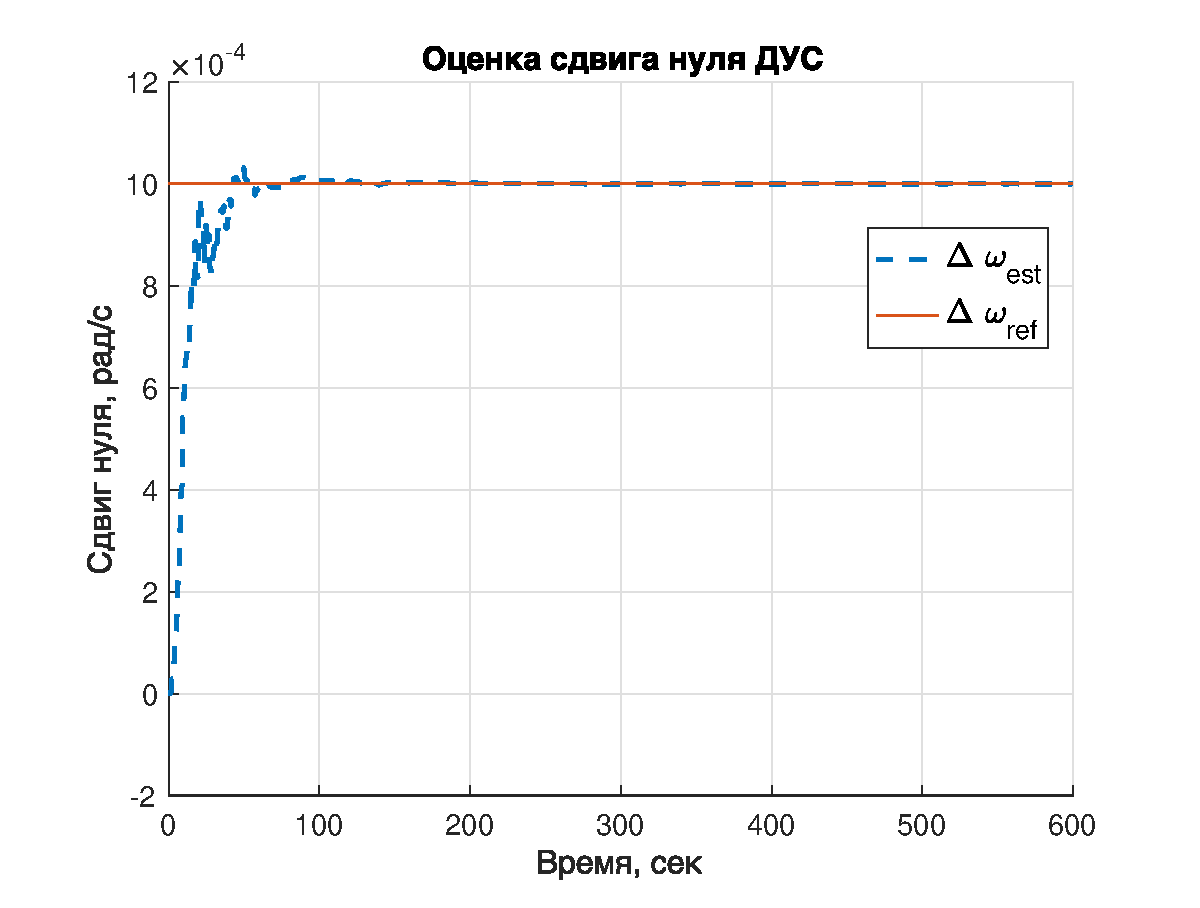
\includegraphics[width=120mm]{gps_gyro_bias.eps}
}
\caption{Оценка ошибок датчика угловой скорости - СНС коррекция}
\label{fig:gps_gyro_bias}
\end{figure}

\clearpage

\subsection{Алгоритм комплексной системы навигации с использованием нелинейного Байесовского фильтра частиц}
Для решения задач оценивания с использованием плотности вероятности распределения оценки произвольного вида (в том числе мультимодальной) и сугубо нелинейных моделей системы и измерений применяется фильтр частиц - Particle Filter (PF), который также является производным от обобщенного Байесовского фильтра.

Фильтр частиц представляет собой непараметрическую реализацию Байесовского фильтра, он  аппрокисмирует плотность вероятности оценки случаной величины набором частиц, представляющих случайные выборки из этой плотности. 

Каждая из множества частиц в PF содержит вектор состояния, оцениваемый фильтром:
\begin{equation}
\chi = \mathbf x_t^{[1]}, \mathbf x_t^{[2]}, \hdots, \mathbf x_t^{[M]};
\end{equation}
где $M$ - общее количество частиц во множестве $\chi$.

Каждая из частиц описывает гипотезу нахождения системы в соответствующей точке пространства состояния и как следствие, чем более плотно ``населена'' соответствующая область в этом пространстве, тем более вероятным является и существование  результирующего вектора оценки в этой области пространства состояния.

Входной информацией для этого алгоритма служит множество частиц $\chi$, вектор измерения $z$ и в общем случае управляющее воздействие $u$. 
В общем случае алгоритм фильтра частиц включает следующие шаги: 
\begin{itemize}
	\item Определение нового вектора состояния для соответствующей частицы на основе предыдущего вектора состояния и текущего управляющего воздействия. Новый вектор состояния для частицы определяется исходя из вероятностной модели системы $ p(x_t|u_t,x_{t-1})$;
	\item Вычисление весового коэффициента $\omega$ для каждой из частиц с помощью текущего вектора измерений $z$ и вероятностной модели измерения $p(z_t|x_t)$;
	\item Выборка нового поколения частиц - чем больше вес частицы, тем с большей вероятностью частица перейдет из текущего поколения в следующее. Выборка производится с замещением, т.е. маловероятные частицы удаляются а высоковероятные дублируются.
\end{itemize}

Из описания алгоритма видно, что фильтр оперирует непосредственно нелинейными вероятностными моделями системы $p(x_t|u_t,x_{t-1})$  и измерений $p(z_t|x_t)$, а распределение плотности вероятности оценки вектора состояния может быть произвольным.

В рамках алгоритма комплексной системы навигации вектор состояния $i$-й частицы имеет следующий вид:
\begin{equation}
 \mathbf x_i = \begin{bmatrix} x_i & y_i & \theta_i  \end{bmatrix}
\end{equation}
где $x_i$, $y_i$ - координаты центра оси колесной пары в навигационной СК, $\theta_i$ - азимутальный угол разворота робота относительно навигационной СК.

Нелинейная модель системы для фильтра частиц определяется моделью кинематики трехколесного робота:
\begin{equation}
 \mathbf x_{i, k} = \begin{bmatrix}  \cos{\theta_{i, k-1}} & 0 \\  \sin{\theta_{i, k-1}} & 0 \\ 0 & 1 \end{bmatrix} \begin{bmatrix} \upsilon^b_x \\ \omega^b_z \end{bmatrix},
\end{equation}
где $ \upsilon^b_x$, $\omega^b_z$ - скорости продольного перемещения и азимутального разворота робота, поступающие в качестве управляющих воздействий от системы траекторного управления колесного робота.

Нелинейная модель измерений для фильтра частиц определяется режимом функционирования локальной радионавигационной системы на базе UWB, доставляющей измерения расстояний между роботом и  базовыми станциями, установленными на соответствующей площадке в рамках которой перемещается робот с установленным на нем приемником системы  UWB:

\begin{equation}
 \mathbf z_{i, k} = \begin{bmatrix} \sqrt{\left(x_{i, k} - x_{UWB, 1}\right)^2 + \left(y_{i, k} - y_{UWB, 1}\right)^2} \\ \vdots \\    \sqrt{\left(x_{i, k} - x_{UWB, n}\right)^2 + \left(y_{i, k} - y_{UWB,  n}\right)^2}  \end{bmatrix} 
\end{equation}
где $x_{UWB, n}$, $y_{UWB, n}$ - координаты $n$-ой базовой станции системы UWB в навигационной СК, $n$ - общее количество базовых станций. 

\subsection{Моделирование работы алгоритма комплексной системы навигации с использованием нелинейного Байесовского фильтра частиц}
Для оценки работы алгоритма было проведено моделирование в рамках которого задавалось перемещение робота, аналогичной представленной на Рис, \ref{fig:uwb_intergated_trajectory}.  
На рисунках \ref{fig:pf_particles} - \ref{fig:pf_heading} представлены результаты моделирования демонстрирующие устойчиво сходящийся процесс оценивания навигационных параметров робота. 

\begin{figure}
\noindent\centering{
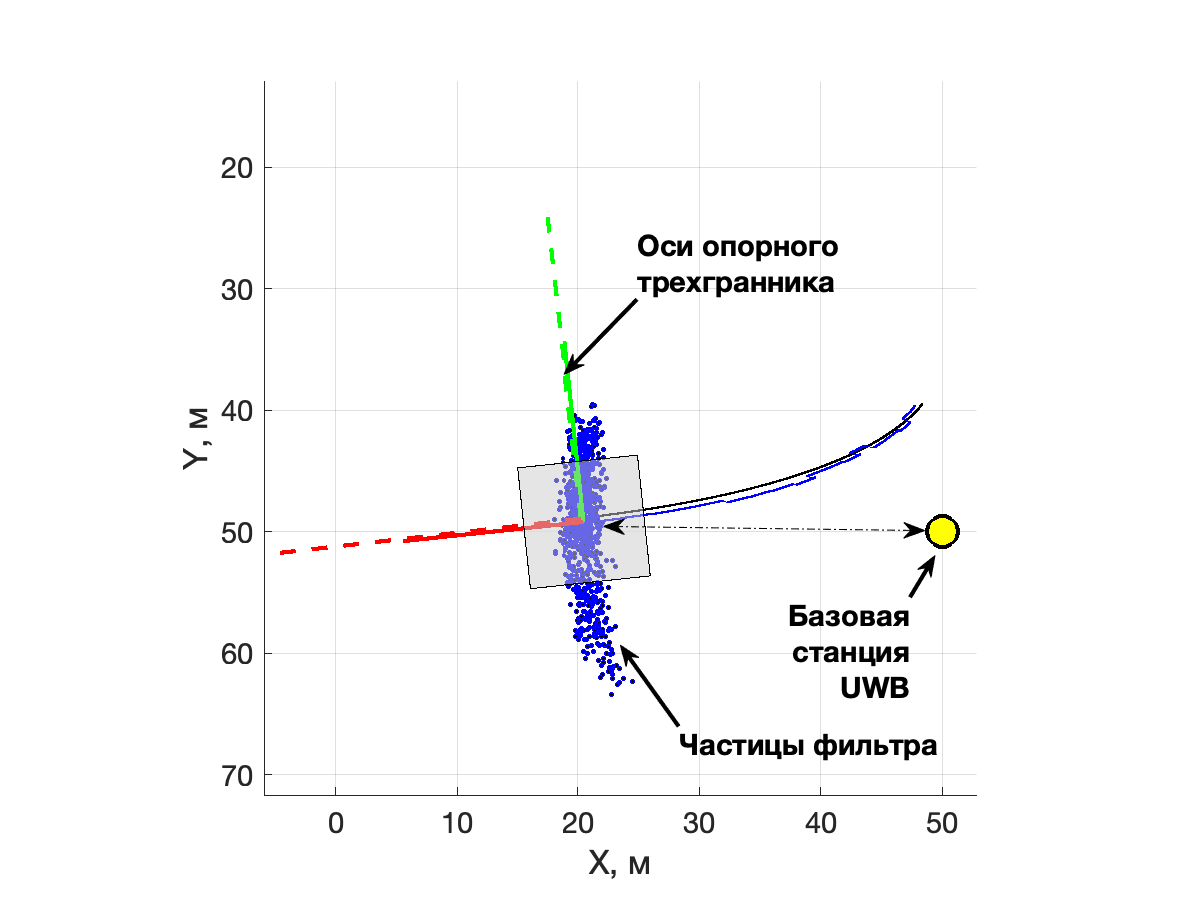
\includegraphics[width=120mm]{uwb_particles.eps}
}
\caption{Пример распределения облака частиц, описывающих плотность вероятности координат робота в навигационной СК}
\label{fig:pf_particles}
\end{figure}

\begin{figure}
\noindent\centering{
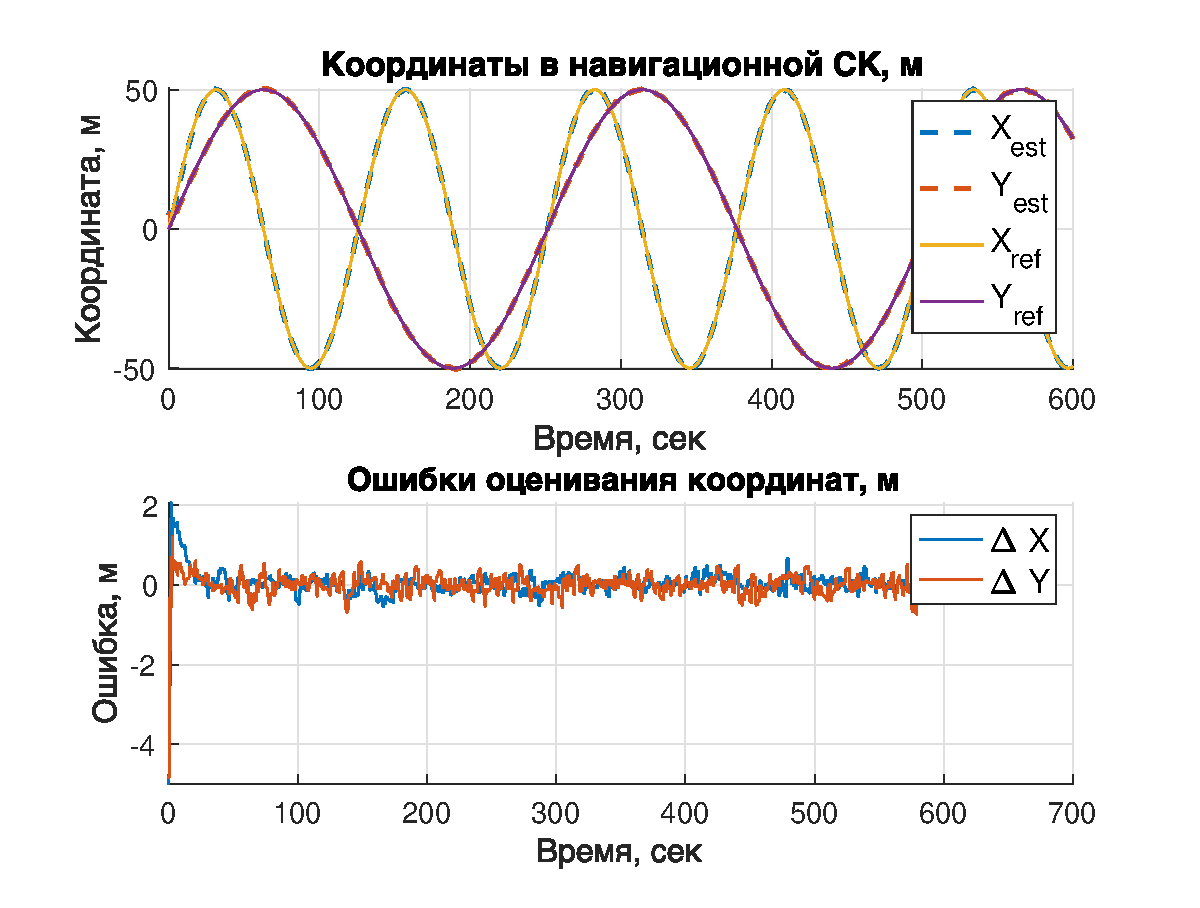
\includegraphics[width=120mm]{uwb_pf_position.eps}
}
\caption{Координаты робота и ошибки их оценок фильтром частиц}
\label{fig:pf_position}
\end{figure}

\begin{figure}
\noindent\centering{
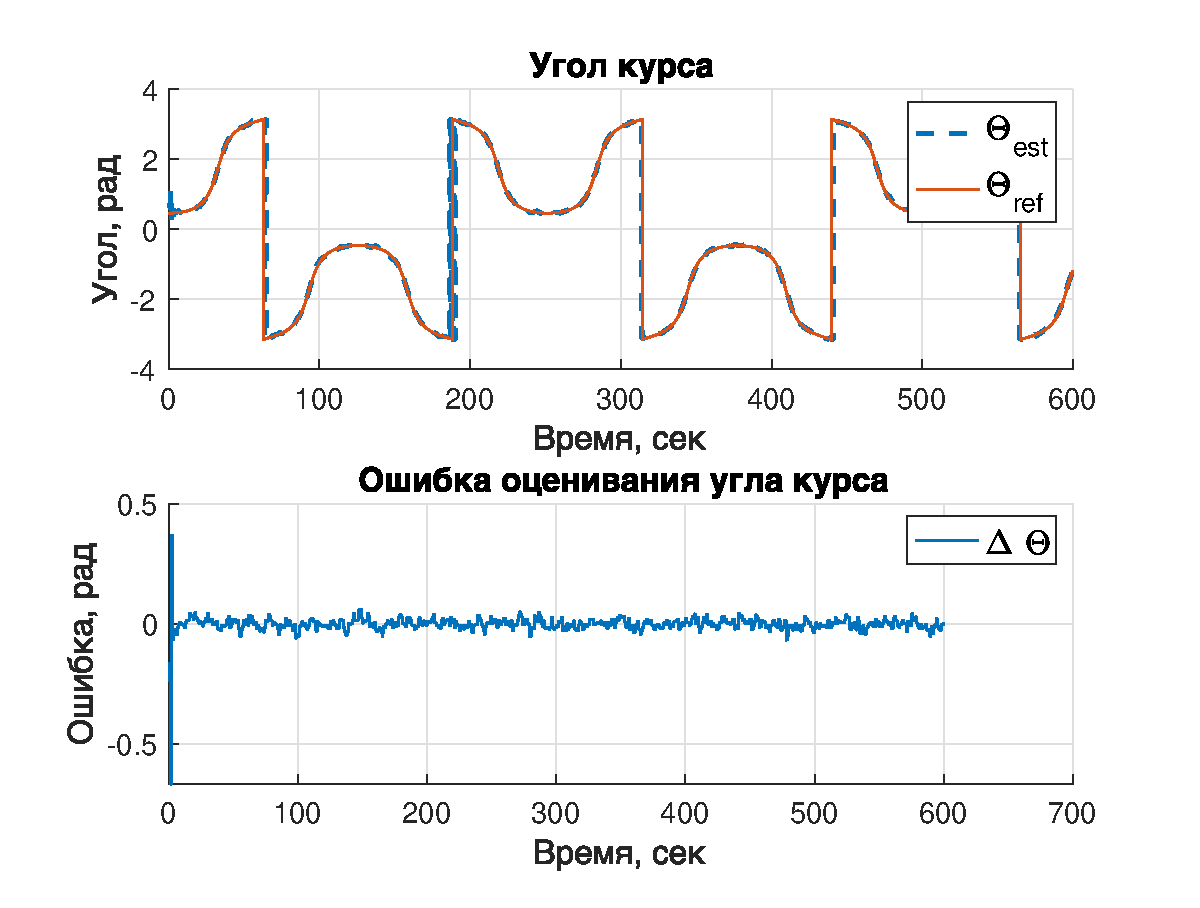
\includegraphics[width=120mm]{uwb_pf_heading.eps}
}
\caption{Угол курса робота и  ошибка его оценки  фильтром частиц}
\label{fig:pf_heading}
\end{figure}

\clearpage

\section{Библиотека алгоритмов обнаружения препятствий - теория}
Для построения алгоритма обнаружения препятствий сделаем несколько допущений (Рис. \ref{fig:axes_tracker}):
\begin{itemize}
\item Примем, что робот оснащен датчиком, доставляющем измерения угла $\gamma$ пеленга (в связанной с роботом системе координат) и дальности $\rho$ до подвижного или неподвижного препятствия;
\item Координаты робота $r_o$ и его угол $\theta$ ориентации в азимуте  поступают от комплексной системы навигации;
\item Известны идентификаторы препятствий - существует однозначный способ сопоставления текущих измерений пеленга и дальности конкретному препятствию.
\end{itemize}

\begin{figure}
\noindent\centering{
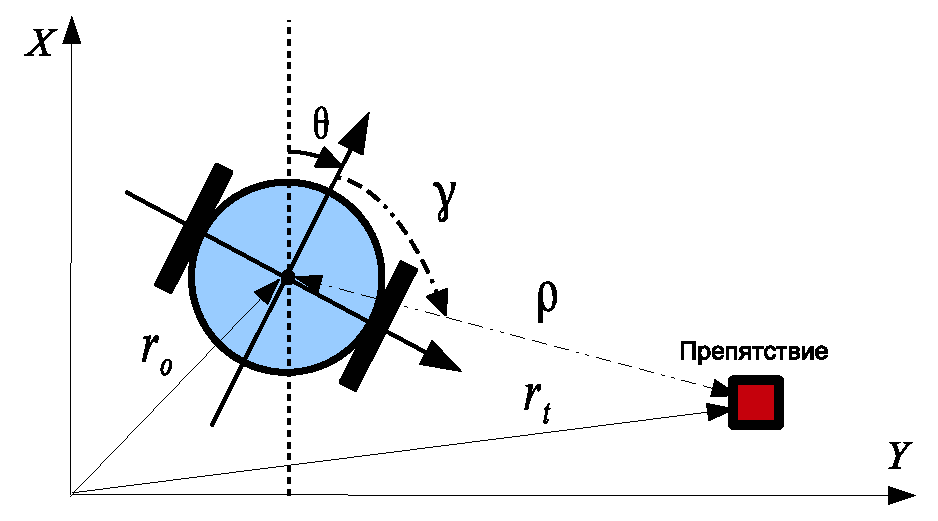
\includegraphics[width=100mm]{axes_tracker.eps}
}
\caption{Конфигурация задачи обнаружения и трекинга препятствий}
\label{fig:axes_tracker}
\end{figure}

Принимая во внимание ряд допущений, приведенных выше, будем строить алгоритм обнаружения препятствий как совокупность индивидуальных алгоритмов-трекеров, построеных на базе расширенного фильтра Калмана (EKF) либо интерактивного многомодельного, расширенного фильтра Калмана (IMM-EKF). 

Верхний уровень архитектуры алгоритма составляет логика в рамках которой каждому наблюдаемому препятствию сопоставляется свой трекер оценивающий координаты и скорости препятствия в навигационной системе координат. При обнаружении и идентификации нового препятствия инициализируется новый трекер, после определенного количества наблюдений препятствие считается захваченным и осуществляется его сопровождение. После пропадания препятствия из вида оценка его координат и скоростей продолжает формироватья в соответствующем трекере до того момента, когда препятсвие считается потерянным. 

Для построения алгоритмов трекеров отдельных препятствий используем алгоритмы, имеющие в своей основе расширенный фильтр Калмана. 

\subsection{Трекер координат и скоростей препятствия на базе EKF}
Задачей трекинга препятствий является задача оценивания их координат и скоростей в навигационной СК. При этом скорости $\dot x, \dot y$  препятствия  не наблюдаются непосредственно, а его координаты связаны с измерением пеленга и дальности нелинейным образом. Поставим задачу оценивания элементов вектора состояния $\boldsymbol x$:
\begin{equation}
	\boldsymbol x = \begin{bmatrix} x & y & \dot x & \dot y \end{bmatrix}^T
\end{equation}

Вектор состояния $\boldsymbol x$ соответствует кинематической модели перемещения материальной точки по плоскости с постоянной скоростью. 

В непрерывной форме уравнение движения точки, перемещающейся по плоскости может быть записано так:
\begin{equation}
	\dot{\boldsymbol x} = A\boldsymbol x + B\boldsymbol \nu
\end{equation}

\begin{equation}\label{equ_6_th_order}
	\dot{\boldsymbol x} = 
	\begin{bmatrix}
		 0 & 0 & 1 & 0 \\
		 0 & 0 & 0 & 1 \\
                 0 & 0 & 0 & 0 \\
                 0 & 0 & 0 & 0 
	 \end{bmatrix}\boldsymbol x + 
	\begin{bmatrix}
		0 & 0 \\ 0 & 0 \\ 1 & 0 \\ 0 & 1
	\end{bmatrix}
	\begin{bmatrix}
		\nu_{\dot x} & 0 \\ 0 & \nu_{\dot y}
	\end{bmatrix}
\end{equation}

где $\nu_x$ и $\nu_y$ - гауссовские шумы ускорений.
\begin{align}
	E\left[\nu(t)\right] &= 0\\
	E\left[\nu(t)\nu(\tau)\right] &= \sigma^2\delta(t-\tau)
\end{align}

Для перехода к дискретной форме записи  уравнений системы с периодом дискретизации $\Delta t$ воспользуемся следующими соотношениями:
\begin{equation}\label{equ_ekf_system_discrete}
\boldsymbol x(k+1) = F\boldsymbol x(k) + \boldsymbol \nu(k)
\end{equation}

\begin{equation}
	F = e^{A\Delta t}
\end{equation}

\begin{equation}
	\boldsymbol\nu(k) = \int_0^{\Delta t}e^{A(\Delta t-\tau)}B\boldsymbol \nu(k\Delta t +\tau)d\tau
\end{equation}

\begin{equation}
	Q = E\left[\boldsymbol \nu(k)\boldsymbol \nu(k)^T\right]
\end{equation}

Тогда для модели \eqref{equ_6_th_order} матрица перехода $F(k)$ и дискретная матрица ковариации $Q(k)$ в дискретной форме запишутся так:
\begin{equation}\label{equ:system_matrix_sixth}
	F(k) = 
	\begin{bmatrix}
		 1 & 0 & \Delta t & 0 \\
		 0 & 1 & 0 & \Delta t \\
                 0 & 0 & 1 & 0\\
                 0 & 0 & 0 & 1
	 \end{bmatrix}
\end{equation}

\begin{equation}
	Q(k) = 
	\begin{bmatrix}
    (\Delta t^3  \sigma)/3 &  0 &   (\Delta t^2 \sigma)/2 &  0 \\
    0 & (\Delta t^3 \sigma)/3 & 0 & (\Delta t^2 \sigma)/2 \\
    (\Delta t^2 \sigma)/2 &  0 &  \Delta t \sigma &  0 \\
    0 & (\Delta t^2 \sigma)/2 & 0 & \Delta t \sigma \\
	 \end{bmatrix}
\end{equation}

Уравнения измерений, связывающие навигационные параметры робота с борта которого осуществляется определение препятствий и координаты препятствия в навигационной СК запишем так:
        
\begin{equation}
f^b = C_n^b \left(r_t^n - r_o^n \right)
\end{equation}      

\begin{equation}
\hat \gamma = \arctan\left( \cfrac{f^b_y}{f^b_x} \right)
\end{equation}    

\begin{equation}
 \hat \rho = ||r_o - r_t||_2
\end{equation}

Вектор измерений $\mathbf z$ и матрица измерений $H$ таковы: 

\begin{equation}
   \mathbf z = 	\begin{bmatrix} \rho - \hat\rho \\ \gamma - \hat\gamma  \end{bmatrix}
\end{equation}

\begin{equation}
   H = \begin{bmatrix}  H_{1, 1} & H_{1, 2} & 0 & 0 \\ H_{2, 1} & H_{2, 2} & 0 & 0  \end{bmatrix}
\end{equation}

\begin{equation*}
H_{1, 1} =  \cfrac{x_o - x_t} {||r_o - r_t||_2}
\end{equation*}

\begin{equation*}
H_{1, 2} =  \cfrac{y_o - y_t} {||r_o - r_t||_2}
\end{equation*}

\begin{equation*}
H_{2, 1} = \cfrac{\partial \gamma}{\partial x_t}
\end{equation*}

\begin{equation*}
H_{2, 2} = \cfrac{\partial \gamma}{\partial y_t}
\end{equation*}


\subsection{Трекер координат и скоростей препятствия на базе IMM-EKF}
Применяемая в предыдущем разделе  кинематическая модель препятствия хотя и является наиболее универсальной, все же не обеспечивает оптимального качества трекинга для неподвижных препятствий, когда нет необходимости использования доступной информации для оценивания скорости препятствия. 

Для различных типов траектории перемещения препятствия оптимальными являются разные кинематические модели, к примеру при прямолинейном перемещении с постоянной скоростью предпочтительно использовать модель четвертого порядка, не включающую ускорения, равные нулю в случае равномерного перемещения, и соответственно не ``тратить'' информацию на их оценивание. Это приводит к улучшению качества трекинга. При маневрировании препятствия предпочтительно использовать кинематическую модель шестого порядка с ускорениями, при координированном развороте (маневр колесного транспортного средства на плоскости) - модель координированного разворота с вектором состояния пятого порядка, включающим координаты, скорости и угловую скорость разворота в азимуте. 

Для решения задачи адаптивного выбора применяется алгоритм IMM EKF (Interactive Multiple Model Extended Kalman Filter).
В таком алгоритме оценка вектора состояния на каждом шаге расчитывается для каждой из $n$ моделей соответствующим EKF фильтром, использующим свою комбинацию оценок векторов состояний, полученных на предыдущем шаге работы алгоритма. Вход для фильтра, соответствующего модели $j$ формируется путем взаимодействия $n$ фильтров, которое заключается в смешивании оценок $\hat{x}^i(k-1|k-1))$ с весовыми коэффициентами (вероятностями) $\mu^{i|j}(k-1|k-1)$, называемыми вероятностями смешивания.

Алгоритм IMM EKF состоит из трех основных этапов, выполняемых на каждом шаге $k$ его работы:
\begin{itemize}
\item Взаимодействие моделей. 

На этом этапе расчитываются вероятности смешивания $\mu^{i|j}_k$ для каждой пары моделей $M^i$ и $M^j$ из дискретного множества моделей $M = \left\{M^1,...,M^n\right\}$:
\begin{align}
	\bar c_j &= \sum_{i=1}^np_{ij}\mu_{k-1}^i\\
	\mu^{i|j}_k &= \cfrac{1}{\bar c_j}p_{ij}\mu_{k-1}^i
\end{align}

где  $\mu^{i|j}_k$ - вероятность модели $M^i$ на шаге $k$, $\bar c_j$ - нормализующий фактор.

Затем расчитываются смешанные входные величины (векторы состояния и матрицы ковариации) для каждого из фильтров по следующим соотношениям:
\begin{align}
	x_{k-1}^{0j} &= \sum_{i=1}^n\mu^{i|j}_kx_{k-1}^i\\
	P_{k-1}^{0j} & = \sum_{i=1}^n\mu^{i|j}_k\left\{P_{k-1}^i+\left[x_{k-1}^i-x_{k-1}^{0j}\right]\left[x_{k-1}^i-x_{k-1}^{0j}\right]^T\right\}
\end{align}

где $m_{k-1}^i$ и $P_{k-1}^i$ - оценки соответственно вектора состояния и матрицы ковариации $i$-ой модели на шаге работы $k-1$.

\item  Фильтрация. 

На этом этапе сначала выполняется собственно фильтрация каждым из фильтров, входящих в состав алгоритма:
\begin{align}
	\left[x_k^{-,i},P_k^{-,i}\right] &= EKF_{predict}\left(x_{k-1}^{0j},P_{k-1}^{0j},F_{k-1}^i,Q_{k-1}^i\right)\\
	\left[x_k^{+,i},P_k^{+,i}\right] &=EKF_{update}\left(x_k^{-,i},P_k^{-,i},z_k,H_k^i,R_k^i\right)
\end{align}

Также вычисляются вероятности измерений для каждого из фильтров:
\begin{equation}
	\Lambda_k^i = N\left(v_k^i,0,S_k^i\right)
\end{equation}

где $v_k^i$ - обновляющая последовательность, $S_k^i$ - матрица ковариации обновляющей последовательности.

Вероятнось для каждой из моделей $M^i$ на шаге $k$ расчитывается как:
\begin{align}
	c &= \sum_{i=1}^n \Lambda_k^i \bar c_i \\
	\mu_k^i &= \cfrac{1}{c}\Lambda_k^i\bar c_i
\end{align}

\item Смешивание оценок.
На последнем этапе работы алгоритма вычисляется комбинированная оценка вектора состояния $\hat{x}_k$  и матрицы ковариации $P_k$:
\begin{align}
	\hat{x}_k &= \sum_{i=1}^n \mu_k^i x_k^i \\
	P_k &= \sum_{i=1}^n \mu_k^i \left\{P_{k}^i+\left[x_{k}^i-x_{k}\right]\left[x_{k}^i-x_{k}\right]^T\right\}
\end{align}
\end{itemize}

В состав набора моделей IMM-EKF для трекинга препятствий включим две модели для подвижного и неподвижного препятствия:
\begin{itemize}
\item Модель четвертого порядка с вектором состояния $\boldsymbol x_1 = \begin{bmatrix} x& y & \dot x & \dot y\end{bmatrix}$;
\item Модель второго порядка с вектором состояния $\boldsymbol x_2 = \begin{bmatrix} x & y\end{bmatrix}$.
\end{itemize}

\subsection{Моделирование работы алгоритма обнаружения препятствий}

\begin{figure}
\noindent\centering{
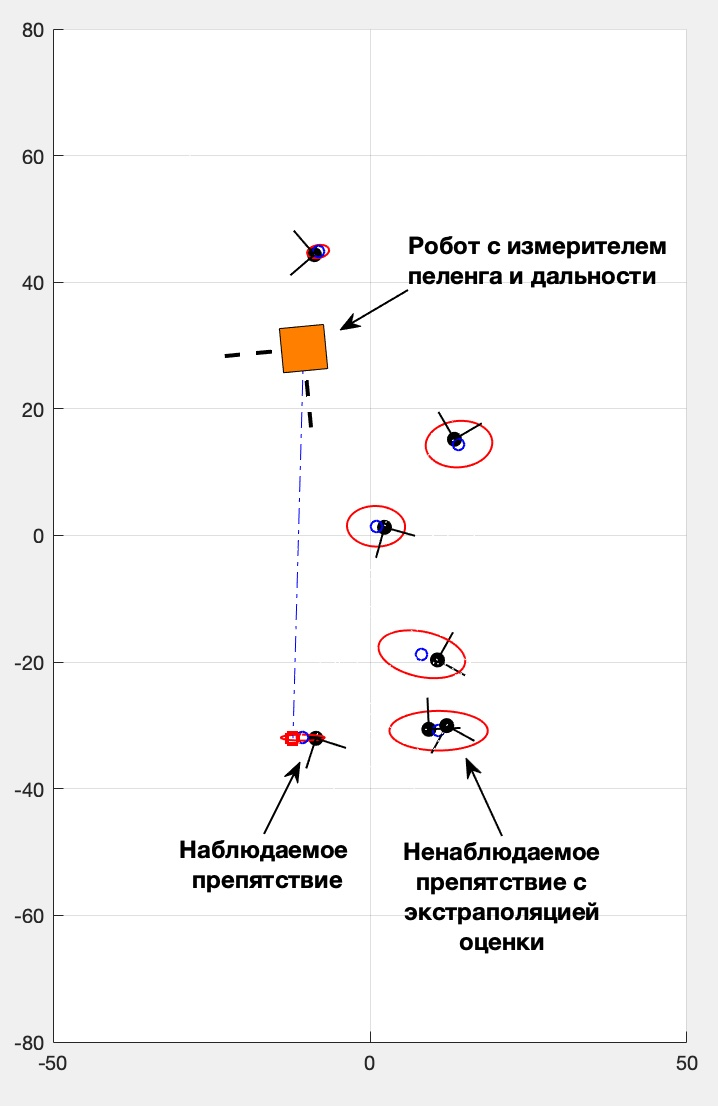
\includegraphics[width=60mm]{tracker_setup.jpeg}
}
\caption{Модельный сценарий задачи обнаружения и трекинга препятствий}
\label{fig:setup_tracker}
\end{figure}

Сценарий моделирования имеет следующие параметры (Рис. \ref{fig:setup_tracker}):

\begin{itemize}
\item Робот-носитель с измерителем пеленга и дальности перемещается по замкнутой траектории;
\item Измеритель пеленга и дальности имеет угол обзора 180 градусов вперед, дальность обнаружения 100 метров. 
\item В области функционирования робота вначале перемещаются, затем становятся стационарными 7 препятствий; 
\end{itemize}

На Рис. \ref{fig:target_tracker} приведены результаты определения алгоритмом координат одного из семи препятствий, различимы момента захвата и трекинга препятствия, экстраполяции оценки его координат на начальном этапе пропадания препятствия из поля зрения измерителя.

\begin{figure}
\noindent\centering{
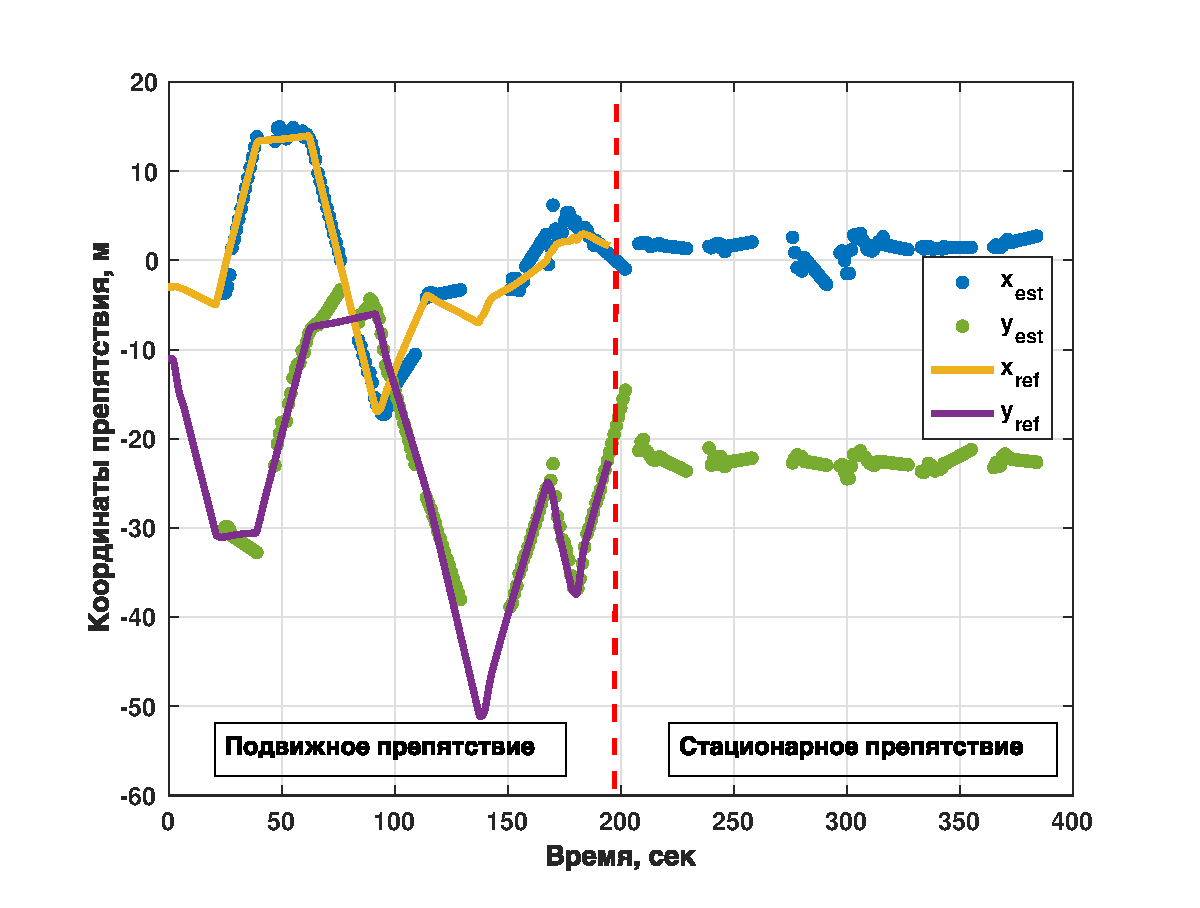
\includegraphics[width=120mm]{target_tracking.eps}
}
\caption{Координаты препятствия и их оценка алгоритмом обнаружения препятствий}
\label{fig:target_tracker}
\end{figure}

\section{Библиотека алгоритмов навигации - программные алгоритмы}
Библиотека алгоритмов навигации разработана на языках программирования Matlab и Python.

\subsection{Алгоритмы ориентации и навигации на базе расширенного фильтра Калмана}

\begin{itemize}
\item Алгоритм гирокомпассирования - Степан


\item Алгоритм курсовертикали.

Реализует алгоритм курсовертикали на базе использования измерений от атчиков угловой скорости, ускорения и магнитного поля.

\begin{verbatim} [Cbn, P, bw] = ahrs_dcm(Cbn, P, bw, dwb, fb, mb, fn, mn, dt) \end{verbatim}

 Входные аргументы: Cbn - матрица направляющих косинусов;  P   - матрица ковариации фильтра Калмана;  bw  - вектор оценок сдвигов нулей ДУС; dwb - вектор измерений ДУС;
fb  - вектор измерений акселерометра; mb  - вектор измерений магнитного поля; fn  - вектор ускорения свободного падения в навигационной СК; mn  - вектор магнитного поля в навигационной СК;
dt  - шаг интегрирования.

Выходные аргументы: Cbn  - матрица направляющих косинусов; P    - матрица ковариации фильтра Калмана bw   - вектор оценок сдвигов нулей ДУС;

\item Алгоритм комплексной системы навигации с коррекцией от СНС.

Реализует процесс оценивания координат, скорости, ошибок датчиков первичной информации для комплексной системы навигации колесного робота, оснащенного одометрами, курсовым гироскопом, приемником СНС.

\begin{verbatim} [rn, Cbn, Vb_odometer, Wb_odometer, P, dw, dlr, dll] = 
navigation_system_GPS
(
  rn, Cbn, P, dt, dThe, fir, fil, lr, ll, d,
  pos_gps, vel_gps, lb, gps_update, dw, dlr, dll
)
 \end{verbatim}
 
 Входные аргументы:  rn - оценка координат робота; Cbn - оценка матрицы направляющих косинусов ориентации робота; P - матрица ковариации фильтра Калмана; dt - шаг интегрирования;
 dThe - измерение приращения угла курса гироскопом за шаг интегрирования; fir - скорость вращения правого колеса; fil - скорость вращения левого колеса; lr - длина окружности правого колеса; 
 ll - длина окружности левого колеса; d - длина оси колесной пары; pos gps - измерение координат приемником GPS, спроецированное в локальную плоскую СК; vel gps - измерение скоростей приемником GPS, спроецированное в локальную плоскую СК; lb - вектор плеча установки приемника GPS относительно центра колесной пары; gps update - индикатор доступности измерения от приемника GPS; 
 dw - оценка сдвига нуля курсового гироскопа; dlr - оценка ошибки длины окружности правого колеса; dll - оценка ошибки длины окружности левого колеса.
 
  Выходные аргументы: rn - оценка координат робота; Cbn - оценка матрицы направляющих косинусов ориентации робота; Vb odometer - оценки скорости продольного перемещения одометром; Wb odometer - оценка скорости курсовго разворота одометром; P - матрица ковариации фильтра Калмана; dw - оценка сдвига нуля курсового гироскопа; dlr - оценка ошибки длины окружности правого колеса; dll - оценка ошибки длины окружности левого колеса.

\item Алгоритм комплексной системы навигации с коррекцией от UWB.

Реализует процесс оценивания координат, скорости, ошибок датчиков первичной информации для комплексной системы навигации колесного робота, оснащенного одометрами, курсовым гироскопом, приемником локальной радионавигационной системы  UWB.

\begin{verbatim}
[rn, Cbn, Vb_odometer, Wb_odometer, P, dlu, dw, dlr, dll, dd] = 
    navigation_system_UWB
    (
    rn, Cbn, P, dt, dThe, fir, fil, lr, ll, d,
    Ranges, Anchors, lu, uwb_update, dlu, dw, dlr, dll, dd
    )
\end{verbatim}

 Входные аргументы: rn - оценка координат робота; Cbn - оценка матрицы направляющих косинусов ориентации робота; P - матрица ковариации фильтра Калмана;
dt - шаг интегрирования; dThe - измерение приращения угла курса гироскопом за шаг интегрирования; fir - скорость вращения правого колеса; fil - скорость вращения левого колеса;
lr - длина окружности правого колеса; ll - длина окружности левого колеса; d - длина оси колесной пары; Ranges - измерения расстояний до базовых станций системы UWB;
Anchors - координаты базовых станций системы UWB; lu - вектор плеча установки приемника UWB относительно центра колесной пары;
uwb update - индикатор доступности измерения от приемника UWB; dlu - оценка ошибки определения плеча установки приемника UWB; dw - оценка сдвига нуля курсового гироскопа;
dlr - оценка ошибки длины окружности правого колеса; dll - оценка ошибки длины окружности левого колеса; dd - оценка ошибки длины оси колесной пары.

Выходные аргументы: rn - оценка координат робота; Cbn - оценка матрицы направляющих косинусов ориентации робота; Vb odometer - оценки скорости продольного перемещения одометром;
Wb odometer - оценка скорости курсовго разворота одометром; P - матрица ковариации фильтра Калмана; dlu - оценка ошибки определения плеча установки приемника UWB;
dw - оценка сдвига нуля курсового гироскопа; dlr - оценка ошибки длины окружности правого колеса; dll - оценка ошибки длины окружности левого колеса;
dd - оценка ошибки длины оси колесной пары. 


\end{itemize}

\subsection{Алгоритм навигации на базе фильтра частиц}

\begin{itemize}
\item Алгоритм локальной радионавигационной системы на базе UWB.

Реализует процесс оценивания координат и угла курса колесноного робота с использованием информации об управляющих воздействиях, поступающих от траекторной системы управления а также с использованием измерений дальностей до локально установленной радиосистемы UWB. 

\begin{verbatim}
[fltr, robot_state] = 
radio_navigation_system_UWB
(
fltr, upsilon, dtheta, Ranges, Anchors, update, dt
)
\end{verbatim}

Входные аргументы: fltr - структура фильтра частиц; upsilon - управляющее воздействие робота - скорость продольного перемещения; dtheta - управляющее воздействие робота - угловая скорость курсового
разворота; Ranges - измерения расстояний до базовых станций системы UWB; Anchors - координаты базовых станций системы UWB; update - индикатор доступности измерения от приемника UWB;
dt - шаг интегрирования.

Выходные аргументы: fltr - структура фильтра частиц; robot state - оценка вектора состояния робота.

\end{itemize}


\section{Библиотека алгоритмов определения препятствий - программные алгоритмы}

Библиотека алгоритмов определения препятствий разработана на языке программирования Matlab.

\begin{itemize}
\item Алгоритм оценивания координат и скоростей препятствий с изменяющейся динамикой движения.

Реализует процесс оценивания коорднат и скоростей множества препятствий, дальность и угол пеленга которых определяется измерителем, устанвленным н подвижном носителе-роботе. Включает в себя базовую логику трекинга, обеспечивающую инициализацию и управление этим процессом за счет использования множества отдельных трекеров на базе алгоритмов EKF и IMM-EKF.

\begin{verbatim}
detector = basic_obstacle_detector
(
detector, rn_platform, Cbn_platform,
targets_range, targets_azimuth, targets_visible
)
\end{verbatim}

Входные аргументы:  detector - структура детектора препятствий с трекерами на базе EKF и IMM; rn platform -  координаты платформы; Cbn platform - углы ориентации платформы;
targets range - дальности до препятствий; targets azimuth - углы пеленга препятствий; targets visible - индикаторы видимости препятствий.

Выходные аргументы: detector - структура детектора препятствий с трекерами на базе EKF и IMM. 

\item Алгоритм трекера на базе EKF.

Реализует процесс оценивания координат и скоростей одного препятствия. Оптимален для подвижного препятствия, движущегося с постоянной скоростью. 

\begin{verbatim}
fltr = ekf_tracker
(
fltr, rn_platform, Cbn_platform, range, azimuth, update
)
\end{verbatim}

 Входные аргументы: fltr - структура EKF фильтра; rn platform -  координаты платформы; Cbn platform - углы ориентации платформы; range - дальность до препятствия;
azimuth - угол пеленга препятствия; update - индикатор включения режима коррекции;

Выходные аргументы: fltr - структура EKF фильтра.

\item Алгоритм трекера на базе IMM-EKF.

Реализует процесс оценивания координат и скоростей одного препятствия. Оптимален для  препятствия с изменяющейся динамикой движения, стационарно-нестационарного.

\begin{verbatim}
fltr = ekf_tracker
(
fltr, rn_platform, Cbn_platform, range, azimuth, update
)
\end{verbatim}

 Входные аргументы: fltr - структура IMM фильтра; rn platform -  координаты платформы; Cbn platform - углы ориентации платформы; range - дальность до препятствия;
azimuth - угол пеленга препятствия; update - индикатор включения режима коррекции;

Выходные аргументы: fltr - структура IMM фильтра.
 

\end{itemize}


\end{document}  